\documentclass[a4paper,12pt]{report}

% Путь до папки с общими шаблонами
\newcommand{\pathToCommonFolder}{../../Common}

% Команда для быстрой вставки названия IDE
\newcommand{\staruml}{StarUML\,\tm}




% Название работы в титуле


% установка размера шрифта для всего документа
%\fontsize{20pt}{18pt}\selectfont
\usepackage{extsizes} % Возможность сделать 14-й шрифт

\author{Кирилл Денисов}
\title{Методические указания по работе c программным обеспечением \staruml}
\date{\today}

% установка полуторного интервала
% \usepackage{setspace}  
% \onehalfspacing


% Вставка заготовки преамбулы
% Этот шаблон документа разработан в 2014 году
% Данилом Фёдоровых (danil@fedorovykh.ru) 
% для использования в курсе 
% <<Документы и презентации в \LaTeX>>, записанном НИУ ВШЭ
% для Coursera.org: http://coursera.org/course/latex .
% Исходная версия шаблона --- 
% https://www.writelatex.com/coursera/latex/5.3

% В этом документе преамбула

% Для корректного использования русских символов в формулах
% пакеты hyperref и настройки, связанные с ним, стоит загуржать
% перед загрузкой пакета mathtext



% поддержка русских букв
% кодировка шрифта
%\usepackage[T2A]{fontenc} 
\usepackage{pscyr}

% использование ненумеровонного абзаца с добавлением его в содержаниеl

\newcommand{\anonsection}[1]{\section*{#1}\addcontentsline{toc}{section}{#1}}
\newcommand{\sectionunderl}[1]{\section*{\underline{#1}}}


% настройка окружения enumerate
\usepackage{enumitem}
\setlist{noitemsep}
\setlist[enumerate]{labelsep=*, leftmargin=1.5pc}

\usepackage{hyperref}

% сначала ставить \usepackage{extsizes} % Возможность сделать 14-й шрифт
% для корректной установки полей вставлять преамбулу следует в последнюю очередь (но перед дерективой замены \rmdefault)
\usepackage[top=20mm,bottom=25mm,left=35mm,right=20mm]{geometry} % Простой способ задавать поля

\hypersetup{				% Гиперссылки
	unicode=true,           % русские буквы в раздела PDF
	pdftitle={Заголовок},   % Заголовок
	pdfauthor={Автор},      % Автор
	pdfsubject={Тема},      % Тема
	pdfcreator={Создатель}, % Создатель
	pdfproducer={Производитель}, % Производитель
	pdfkeywords={keyword1} {key2} {key3}, % Ключевые слова
	colorlinks=true,       	% false: ссылки в рамках; true: цветные ссылки
	linkcolor=red,          % внутренние ссылки
	citecolor=black,        % на библиографию
	filecolor=magenta,      % на файлы
	urlcolor=blue           % на URL
}

%%% Работа с русским языком
\usepackage{cmap}					% поиск в PDF
\usepackage{mathtext} 				% русские буквы в формулах
\usepackage[T2A]{fontenc}			% кодировка
\usepackage[utf8]{inputenc}			% кодировка исходного текста
\usepackage[english,russian]{babel}	% локализация и переносы
\usepackage{indentfirst}
\frenchspacing

%для изменения названия списка иллюстраций
\usepackage{tocloft}


\renewcommand{\epsilon}{\ensuremath{\varepsilon}}
\renewcommand{\phi}{\ensuremath{\varphi}}
\renewcommand{\kappa}{\ensuremath{\varkappa}}
\renewcommand{\le}{\ensuremath{\leqslant}}
\renewcommand{\leq}{\ensuremath{\leqslant}}
\renewcommand{\ge}{\ensuremath{\geqslant}}
\renewcommand{\geq}{\ensuremath{\geqslant}}
\renewcommand{\emptyset}{\varnothing}

% Изменения параметров списка иллюстраций
\renewcommand{\cftfigfont}{Рисунок } % добавляем везде "Рисунок" перед номером
\addto\captionsrussian{\renewcommand\listfigurename{Список иллюстративного материала}}

\newcommand{\tm}{\texttrademark\ }
\newcommand{\reg}{\textregistered\ }


%%% Дополнительная работа с математикой
\usepackage{amsmath,amsfonts,amssymb,amsthm,mathtools} % AMS
\usepackage{icomma} % "Умная" запятая: $0,2$ --- число, $0, 2$ --- перечисление

%% Номера формул
%\mathtoolsset{showonlyrefs=true} % Показывать номера только у тех формул, на которые есть \eqref{} в тексте.
%\usepackage{leqno} % Нумереация формул слева

%% Свои команды
\DeclareMathOperator{\sgn}{\mathop{sgn}}

%% Перенос знаков в формулах (по Львовскому)
\newcommand*{\hm}[1]{#1\nobreak\discretionary{}
{\hbox{$\mathsurround=0pt #1$}}{}}


% отступ для первого абзаца главы или параграфа
%\usepackage{indentfirst}

%%% Работа с картинками
\usepackage{graphicx}  % Для вставки рисунков
\graphicspath{{images/}{screnshots/}}  % папки с картинками
\DeclareGraphicsExtensions{.pdf,.png,.jpg}
\setlength\fboxsep{3pt} % Отступ рамки \fbox{} от рисунка
\setlength\fboxrule{1pt} % Толщина линий рамки \fbox{}
\usepackage{wrapfig} % Обтекание рисунков текстом

%%% Работа с таблицами
\usepackage{array,tabularx,tabulary,booktabs} % Дополнительная работа с таблицами
\usepackage{longtable}  % Длинные таблицы
\usepackage{multirow} % Слияние строк в таблице

%%% Теоремы
\theoremstyle{plain} % Это стиль по умолчанию, его можно не переопределять.
\newtheorem{theorem}{Теорема}[section]
\newtheorem{proposition}[theorem]{Утверждение}

\theoremstyle{plain} % Это стиль по умолчанию, его можно не переопределять.
\newtheorem{work}{Практическая работа}[part]


 
 
\theoremstyle{definition} % "Определение"
\newtheorem{corollary}{Следствие}[theorem]
\newtheorem{problem}{Задача}[section]
 
\theoremstyle{remark} % "Примечание"
\newtheorem*{nonum}{Решение}



%%% Программирование
\usepackage{etoolbox} % логические операторы

%%% Страница

%	\usepackage{fancyhdr} % Колонтитулы
% 	\pagestyle{fancy}
%   \renewcommand{\headrulewidth}{0pt}  % Толщина линейки, отчеркивающей верхний колонтитул
% 	\lfoot{Нижний левый}
% 	\rfoot{Нижний правый}
% 	\rhead{Верхний правый}
% 	\chead{Верхний в центре}
% 	\lhead{Верхний левый}
%	\cfoot{Нижний в центре} % По умолчанию здесь номер страницы

\usepackage{setspace} % Интерлиньяж
\onehalfspacing % Интерлиньяж 1.5
%\doublespacing % Интерлиньяж 2
%\singlespacing % Интерлиньяж 1

\usepackage{lastpage} % Узнать, сколько всего страниц в документе.

\usepackage{soul} % Модификаторы начертания


\usepackage[usenames,dvipsnames,svgnames,table,rgb]{xcolor}


\usepackage{csquotes} % Еще инструменты для ссылок

%\usepackage[style=authoryear,maxcitenames=2,backend=biber,sorting=nty]{biblatex}

\usepackage{multicol} % Несколько колонок

\usepackage{tikz} % Работа с графикой
\usepackage{pgfplots}
\usepackage{pgfplotstable}

% модуль для вставки рыбы
\usepackage{blindtext}

\usepackage{listings}
\usepackage{color}


% для поворота отдельной страницы. Использовать окружение \landscape
\usepackage{pdflscape} 
\usepackage{rotating} 


\definecolor{mygreen}{rgb}{0,0.6,0}
\definecolor{mygray}{rgb}{0.5,0.5,0.5}
\definecolor{mymauve}{rgb}{0.58,0,0.82}


% пример импорта файла
%\lstinputlisting{/home/denilai/repomy/conf/distributions}

\lstset{
	language=Python,
	basicstyle=\footnotesize,        % the size of the fonts that are used for the code
	numbers=left,                    % where to put the line-numbers; possible values are (none, left, right)
	numbersep=5pt,                   % how far the line-numbers are from the code
	numberstyle=\tiny\color{mygray}, % the style that is used for the line-numbers
	stepnumber=2,                    % the step between two line-numbers. If it's 1, each line will be numbered
	% Tab - 2 пробела
	tabsize=2,    
	% Автоматический перенос строк
	breaklines=true,
	frame=single,
	breakatwhitespace=true,
	title=\lstname 
}





%\renewcommand{\cftloftitlefont}{\hspace{0.38\textwidth}\MakeTextUppercase} % в верхнем регистре
% использовать Times New Roman
\renewcommand{\rmdefault}{ftm}

\begin{document}
\maketitle
\newpage

% Тут я добавляю в содержание
	%\thispagestyle{empty}
	
	% Вставка первого титульного листа
	%%\newcounter{withouttheme}

%\setcounter{withouttheme}{<n>} установить значение счетчика  withouttheme для определения, нужна ли тема
%    {0} - нужна
%    {1} - не нужна

%\setcounter{withoutsubmissiondate}{<n>} установить значение счетчика  withoutsubmissiondate для определения, нужна ли дата представления к защите
%     {0} - нужна
%     {1} - не нужена
\begin{center}
	\begin{figure}[h!]
		\begin{center}
		%\vspace{-10ex}
		
\includegraphics[width=0.17\linewidth]{\pathToCommonFolder/gerb}
		%\caption{}\label{pic:first}
		%	\vspace{5ex}
		\end{center}	
	\end{figure}
 	\small	МИНОБРНАУКИ РОССИИ \\
	Федеральное государственное бюджетное образовательное учреждение\\
						высшего образования\\
\normalsize					
\textbf{«МИРЭА – Российский технологический университет»\\
						РТУ МИРЭА}\\
						\noindent\rule{1\linewidth}{1pt}\\
       Институт информационных технологий\\ %\vspace{2ex}
					\kafedra\\
		\vspace{3ex}
			\large \textbf{\workname}  \\
		%\vspace{1ex}
						по дисциплине\\ «\discipline» \\
		\vspace{3ex}
		\ifnum \value{withouttheme}=0 {
			\textbf{Тема работы:}\\ <<\theme>>
		}
		\else {}
		\fi
\vspace{10ex}
\small
\begin{table}[h!]
\begin{tabular}{lp{0.6\linewidth}l}
	\textbf{Выполнил:} & студент группы ИВБО-02-19 & \\ 
	& & \studentfio \\%Д.~Н.~Федосеев\\%А.~М.~Сосунов\\%К.~Ю.~Денисов\\%И.~А.~Кремнев
	\textbf{Принял:} & \rang & \\
	& & \teacherfio \hfill\\
\end{tabular}
\end{table}
\end{center}
\ifnum \value{withoutsubmissiondate}=0 {
	\begin{flushleft}
		Работа представлена к защите <<\rule{3ex}{1pt}>>\rule{10ex}{1pt} 202\rule{1ex}{1pt} г.\hfill
	\end{flushleft}
\else {}
\fi

\normalsize
\begin{center}	
\vfill
Москва 2022
\end{center}

	\newpage
	\tableofcontents
	\newpage

	
	\newpage
	
	
\chapter{Краткий обзор \staruml}

\staruml --- программный инструмент моделирования, который поддерживает UML
(Унифицированный язык моделирования). \staruml ориентирован на UML версии 1.4 и
поддерживает одиннадцать различных типов диаграмм, принятых в нотации UML 2.0. Он активно
поддерживает подход MDA (Модельно-управляемая архитектура), реализуя концепцию профилей
UML. Среда разработки \staruml превосходно настраивается в соответствии с требованиями
пользователя и имеет высокую степень расширяемости, особенно в области своих
функциональных возможностей. Использование \staruml, одного из ведущих программных
инструментов моделирования, гарантирует достижение максимальной производительности и
качества ваших программных проектов.
\subsection*{Инструмент UML, который адаптируется к пользователю}
\staruml  предоставляет максимальную степень адаптации среды разработки пользователя,
предлагая настройку параметров, которые могут влиять на методологию разработки программного
обеспечения, проектную платформу и язык.

\subsection*{Превосходная расширяемость и гибкость}
\staruml  обеспечивает превосходную расширяемость и гибкость. Он предоставляет механизм
аддинов, чтобы расширять свои функциональные возможности. Этот механизм разработан
специально, чтобы предоставлять доступ ко всем функциям модели/мета-модели посредством
COM Automation и расширять меню и набор свойств элементов. Также, пользователи могут
создавать собственные подходы и механизмы согласно своим собственным методологиям.
Программа может также быть интегрирована с любыми внешними инструментальными
средствами.

\subsection*{Системные требования}
Ниже указаны минимальные системные требования, необходимые для функционирования
\staruml.
\begin{itemize}
	\item Intel \reg Pentium \reg 233MHz или выше
	\item Windows \reg 2000, Windows XP TM, или выше
	\item Microsoft \reg Internet Explorer 5.0 или выше
	\item 128 Мбайт RAM (256 МБ рекомендуется)
	\item 110 Мбайт на жестком диске (150 МБ рекомендуется)
	\item Устройство CD-ROM
	\item SVGA или монитор с более высокой разрешающей способностью (1024x768 рекомендуется)
	\item Мышь или другое устройство позиционирования
\end{itemize}
\chapter{Основные концепции}
Эта глава вводит фундаментальные концепции, которые требуется знать для эффективного
использования \staruml. Она содержит описание моделей, визуальных элементов и диаграмм,
проектов, секций, подходов, фреймворков, модельных фрагментов, их различий относительно
разных профилей UML.
\begin{itemize}
	\item Модель,
	\item Представление (view) и Диаграмма
	\item Проект и проектная секция (unit)
	\item Модуль (module)
\end{itemize}

\sectionunderl{Модель, Представление и Диаграмма}
% TODO: \usepackage{graphicx} required
\begin{figure}[h!]
	\centering
	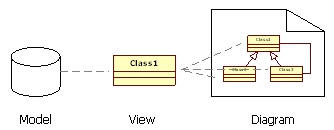
\includegraphics[width=0.7\linewidth]{images/modelviewdiagram}
	\caption{Модель, представление, диаграмма}
	\label{fig:modelviewdiagram}
\end{figure}
\staruml предполагает ясное понимание концептуального различия между моделями,
представлениями и диаграммами. Модель --- элемент, который содержит всю информацию о модели
программы. Представление --- визуальное выражение информации, содержавшейся в модели, а
Диаграмма --- коллекция визуальных образов, которая отображает определенные аспекты проекта.

\sectionunderl{Проект и проектная секция}
\subsection*{Проект}
Проект -- основная структурная единица в \staruml.
Проект может содержать одну или более программных моделей. Проект - корневой пакет
верхнего уровня, который всегда существует в любой программной модели. В общем случае, один
проект сохраняется в одном файле.

\subsection*{Структура проекта}
Проект содержит следующие суб-элементы:

Модель --- элемент, который соответствует одной программной модели.

Подсистема --- элемент, который соответствует модели подсистемы.

Пакет --- самый общий элемент для группировки других элементов.

\subsection*{Проектный файл}Проектные файлы сохраняются в формате XML и имеют расширение \textit{".UML"}. Все модели,
представления и диаграммы, созданные в \staruml сохраняются в одном проектном файле.
Проект может также быть разделен и сохранен в нескольких проектных секциях. Проектный файл
содержит следующую информацию:
\begin{itemize}
	\item профиль UML, используемый в проекте
	\item файлы секций, на которые ссылается проект
	\item информация по всем моделям, содержавшимся в проекте
	\item информация по всем диаграмм и представлениям, содержавшимся в проекте
\end{itemize}


\subsection*{Секции}
Хотя проект обычно сохраняется в одном файле, бывают случаи, когда его целесообразно
хранить в нескольких небольших файлах так, чтобы несколько разработчиков могли работать над
проектом одновременно. В этом случае, проект представляется в виде набора секций. Секция
может иметь иерархическую структуру; она может содержать несколько подсекций. Секции
сохраняются как XML-файлы на которые ссылаются проектные файлы (.UML) или другие файлы
секций (.UNT).
\subsection*{Состав секции}
Только пакет, подсистема или модель могут составлять секцию. Все элементы внутри пакетов
этих типов сохраняются в соответствующем файле секции (.UNT).
\subsection*{Иерархическая структура секции}
Также, как проект может содержать много секций внутри себя, секция тоже может включать
много подсекций. Так как родительская секция имеет ссылки на свои дочерние секции, всё
множество секций имеет иерархическую структуру.
\subsection*{Фрагменты модели}
Фрагмент модели --- часть проекта, сохраненная как отдельный файл. Только модель, подсистема
или пакет может являться фрагментом модели. Файлы модельных фрагментов сохраняются с
расширением <<.MFG>>. Они могут быть легко включены в любой проект в любое время. Фрагменты
модели существенно отличаются от секций, которые полностью едины с остальной частью
проекта.

\chapter{Управление проектом}
Эта глава подробно описывает операции по управлению проектом: создание нового проекта,
размещение части проекта в секции, создание и импорт фрагментов модели, импорт фреймворков,
подключение и исключение профилей UML.
\begin{itemize}
	\item Управление проектом
	\item Управление секциями
	\item Работа с фрагментами модели
	\item Импорт фреймворка
	\item Работа с профилями UML
\end{itemize}

\sectionunderl{Управление проектом}
\subsection*{Создание нового проекта}
Чтобы начать разработку программного обеспечения, нужно инициировать новый проект. Вы
можете начать абсолютно пустой проект или инициализировать новый проект согласно
определённому подходу.

\subsubsection*{Процедура создания нового проекта \#1 --- New Project:}
\begin{enumerate}
	\item выберите меню [File] -> [New Project].
	\item Новый проект будет создан в соответствии с подходом по умолчанию, ранее выбранным
	пользователем. В зависимости от подхода могут быть подгружены определённые профили
	и/или инструментарии.
\end{enumerate}
 
\subsubsection*{Процедура создания нового проекта \#2 --- Select Select New Project}
\begin{enumerate}
	\item Выберите меню [File] -> [Select New Project...].
	диалоговом окне New Project будет отображен список доступных подходов.
	\item Выберите	нужный из списка и нажмите кнопку [OK].
	\item Новый проект будет создан и инициализирован согласно указанному подходу. В
	зависимости от подхода могут быть подгружены определённые профили и/или фреймворки.
\end{enumerate}

\paragraph{Примечание}
\begin{itemize}
	\item Список доступных подходов зависит от инсталлированной среды разработки пользователя.
	\item Чтобы изменить заданный по умолчанию подход, откройте диалоговое окно "Select New
	Project", выберите нужный подход и затем установите опцию "Set As Default Approach"
	(Использовать как подход по умолчанию).
\end{itemize}

\subsection*{Открытие проекта}
Чтобы начать работать с существующим проектом, его проектный файл нужно открыть. Если
проект включает более одной секции, все связанные секции будут также загружены вместе с
проектом.

\subsubsection*{Процедура открытия проекта:}
\begin{enumerate}
	\item Выберите меню [File] -> [Open...].
	\item В диалоговом окне "Open Project", выберите файл проекта (.UML) и нажмите кнопку
	[Open].
	\item Выбранный проектный файл будет открыт.
\end{enumerate}

\paragraph{Примечание}
Проекты могут также быть открыты через диалоговое окно "Select New Project".

\subsection*{Сохранение проекта}
Чтобы изменения, сделанные в проекте, не пропали, проектный файл должен быть должным
образом сохранен. Ваша работа может быть сохранена в существующий проектный файл или в 
новый проектный файл. Когда проектный файл сохраняется, то вместе с ним сохраняются данные
из связанных с ним секций.
\subsubsection*{Процедура сохранения проекта:}
\begin{enumerate}
	\item Выберите меню [File] -> [Save].
	\item Если имя файла проекта не было определено, появится диалоговое окно "Save Project".
	Введите имя файла, и нажмите кнопку [Save].
	\item Проектный файл будет сохранен.
\end{enumerate}


% TODO: \usepackage{graphicx} required
\begin{figure}[h!]
	\centering
	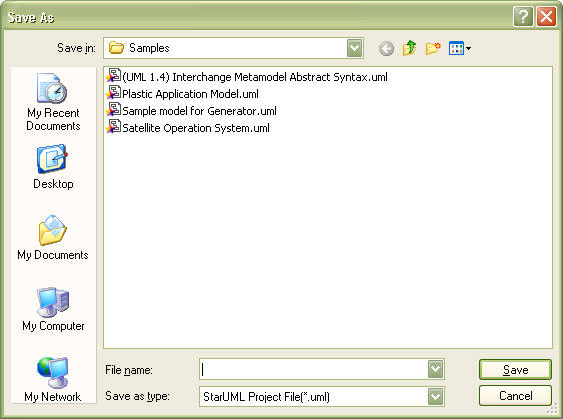
\includegraphics[width=0.5\linewidth]{images/saveproject}
	\caption{Сохранение проекта}
	\label{fig:saveproject}
\end{figure}



\subsubsection*{Процедура сохранения проекта в новом файле:}
\begin{enumerate}
	\item Выберите меню [File] -> [Save As...].
	\item В диалоговом окне <<Save As>>, введите новое имя файла, и нажмите кнопку [Save].
	\item Проект будет сохранен в указанном файле.
\end{enumerate}

\paragraph{Примечание}
\begin{itemize}
	\item Если проект содержит одну или более секций, и есть изменённые секции, диалоговое окно
	будет запрашивать подтверждение на сохранение каждой измененной секции. Выберите
	[Yes], чтобы сохранить измененную секцию вместе с проектом.
\end{itemize}

\subsection*{Закрытие проекта}
Проект может быть закрыт, если больше не требуется его редактирование.
\subsubsection*{Процедура закрытия проекта:}
\begin{enumerate}
	\item Выберите меню [Файл]->[Close].
	\item Если проект не был сохранен после внесения изменений, пользователю будет предложено
	сохранить изменения. Пользователь может выбрать <<да>>, <<нет>> или <<отмена>>.
	\item После закрытия проект становится недоступным для редактирования.
\end{enumerate}

% TODO: \usepackage{graphicx} required
\begin{figure}[h!]
	\centering
	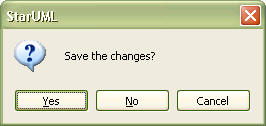
\includegraphics[width=0.4\linewidth]{images/closeproject1}
	\caption{Закрытие проекта}
	\label{fig:closeproject1}
\end{figure}



\subsection*{Управление элементами с помощью моделей, подсистем и пакетов}
Программная модель состоит из многих элементов и диаграмм. Правильная группировка этих
элементов и диаграмм очень важна для эффективного управления проектом. \staruml
поддерживает три типа группирующих элементов (модели, подсистемы и пакеты), которые
пользователь может использовать соответственно их назначению.
Способы группировки элементов, реализованные в \staruml.



\includegraphics[width=3ex]{images/folder}Модель

Модель выражает физическую систему в определенном аспекте. Например, это может быть аспект
анализа, аспект проекта, пользовательский аспект, и т.д.

% TODO: \usepackage{graphicx} required

\includegraphics[width=3ex]{images/subsistem}
Подсистема

Подсистема группирует элементы, которые составляют полную физическую систему или её части.

% TODO: \usepackage{graphicx} required

\includegraphics[width=3ex]{images/package}
Пакет

Пакет логически группирует и содержит модельные элементы. Это чрезвычайно обобщенный
элемент, который может использоваться только для того, чтобы как-то организовать модельные
элементы.

\chapter{Моделирование с помощью \staruml}
Эта глава подробно описывает, как создавать и редактировать элементы диаграммы, включая
способы организации структуры модели с помощью навигатора модели.
\begin{itemize}
	\item Редактирование элементов и диаграмм
	\item Организация структуры модели
\end{itemize}

\sectionunderl{Редактирование элементов и диаграмм}
\subsection*{Создание новой диаграммы}
\staruml TM поддерживает 11 типов диаграмм UML. Пользователь может свободно создавать и
манипулировать диаграммами различных типов, как ему необходимо.
\subsubsection*{Процедура создания новой диаграммы:}
\begin{enumerate}
	\item Выберите в навигаторе модели или на диаграмме элемент, который будет содержать новую
	диаграмму.
	\item Щелкните правой кнопкой мыши и выберите [Add Diagram]. Новая диаграмма будет
	создана после выбора типа диаграммы.
\end{enumerate}

\subsubsection*{Доступные типы диаграмм}
\begin{itemize}
 
\item \textbf{Диаграмма классов (Сlass diagram)}

Диаграмма классов - визуальное отображение различных статических отношений между
класс-подобными элементами. Диаграмма классов может содержать не только классы, но
также и интерфейсы, перечислимые типы, пакеты, различные отношения, инстанции и их
связи.
\item \textbf{Диаграмма прецедентов (Use case diagram)}

Диаграмма прецедентов - отображение отношений между вариантами использования
(прецедентами) определенной системы или объекта и внешними акторами. Вариант
использования отображает функции системы и то, как эти функции взаимодействуют с
внешними акторами.
\item \textbf{Диаграмма сообщений (Sequence Diagram)}

Диаграмма сообщений отображает взаимодействие инстанций. Она является прямым отображением множества взаимных воздействий (InteractionInstanceSet) между элементами
множества инстанций (CollaborationInstanceSet). В то время как Диаграмма сообщений роли
ориентирована на классификаторы-роли, обычная Диаграмма сообщений - на инстанции.
\item \textbf{Диаграмма сообщений роли (Sequence Role Diagram)}

Диаграмма сообщений роли отображает взаимодействия в концепции ролей. Она является
прямым отображением Interaction (множества взаимных сообщений между
классификаторами-ролями) в пределах Collaboration. В то время как Диаграмма сообщений
- отображение инстанций, Диаграмма сообщений роли - отображение классификаторов-
ролей.
\item \textbf{Диаграмма коллаборации (Collaboration Diagram)}

 Диаграмма коллаборации отображает взаимодействие между инстанциями. Она является
прямым отображением модели взаимодействия инстанций, входящих в CollaborationInstanceSet. В то время как диаграмма коллаборации ролей - отображение
классификаторов-ролей, обычная диаграмма коллаборации - отображение инстанций.
\item \textbf{Диаграмма коллаборации ролей}

Диаграмма коллаборации ролей отображает взаимодействия между ролями. Она является
прямым отображением модели взаимодействия классификаторов-ролей внутри
коллаборации. В то время как обычная диаграмма коллаборации ориентирована на
отображение инстанций, диаграмма коллаборации ролей - отображение классификаторов-
ролей.
\item\textbf{ Диаграмма состояний (Statechart Diagram)}

Диаграмма состояний выражает статическое поведение определенного объекта через
состояния и переходы состояний. Хотя диаграмма состояний обычно используется, чтобы
выразить поведение инстанций классов, она может также использоваться, чтобы выражать
поведение и других элементов.
\item \textbf{Диаграмма действий (Activity Diagram)}

Диаграмма действий - специальная форма диаграммы состояний, которая является
подходящей для того, чтобы отображать поток выполнения действий. Диаграмма действий в
общем случае используется для отображения любых потоков обработки, но чаще всего
применительно к объектам подобным классам, пакетам и операциям.
\item \textbf{Диаграмма компонентов (Component Diagram)}

Диаграмма компонентов отображает зависимость между программными компонентами.
Элементы, которые составляют программные компоненты и элементы, которые реализуют
эти компоненты, могут быть отображены на диаграмме компонентов.
\item \textbf{Диаграмма развертывания (Deployment Diagram)}

Диаграмма развертывания отображает аппаратные элементы компьютера, другие
устройства и программные компоненты, а также процессы и объекты, которые им
назначены.
\item \textbf{Композиционная структурная диаграмма (Composite Structure Diagram)}

Композиционная структурная диаграмма - диаграмма, выражающая внутреннюю структуру
классификатора. Она показывает его точки зрения взаимодействия с другими частями
системы.

\end{itemize}
\paragraph*{Примечание}
\begin{itemize}
	\item Типы доступных диаграмм изменяются при переходе от одного типа элемента к другому.
\end{itemize}
\subsection*{Создание элемента на диаграмме}
Чтобы создать на диаграмме новый элемент, диаграмму сначала нужно открыть. Палитра
элементов содержит различные типы элементов, доступных для создания в зависимости от типа
диаграммы. Список доступных элементов изменяется при переходе от диаграммы одного типа к
диаграмме другого типа.


\subsubsection*{Процедура создания элемента из палитры элементов:}
\begin{enumerate}
	\item Выберите тип создаваемого элемента на палитре элементов.
	\item Щёлкните желаемое место для нового элемента на диаграмме, чтобы создать там элемент.
	(Перетаскивайте указатель мыши, чтобы определить область и размер нового элемента. При
	создании элемента, который соединяет два других элемента, убедитесь, что соединение
	сделано правильно.)
\end{enumerate}

\subsubsection*{Процедура одновременного создания нескольких однотипных элементов:}
\begin{enumerate}
	\item Выберите тип создаваемого элемента на палитре элементов.
	\item Нажмите [Lock] на палитре или тот же тип элемента еще раз.
	\item Создайте несколько элементов подряд.
	\item Снова нажмите элемент в палитре, когда создание группы элементов будет закончено.
\end{enumerate}

\paragraph{Примечание}
\begin{itemize}
	\item Создание элемента на диаграмме с помощью палитры элементов фактически означает
	создание как собственно модельного элемента, так и его визуального образа.
\end{itemize}


\subsection*{Редактирование элемента на диаграмме}
Элементы могут редактироваться непосредственно на диаграмме.
\subsubsection*{Процедура редактирования элемента:}
\begin{enumerate}
	\item Дважды щелкните образ на диаграмме.
	\item В "горячем диалоге" редактируйте имя элемента, область видимости и т.д., или нажмите
	кнопку, чтобы создать подчинённые элементы для выбранного элемента.
	\item Нажмите [Enter] или щёлкните другое место на диаграмме, чтобы принять изменения.
\end{enumerate}

\paragraph{Примечание}
\begin{itemize}
	\item Для детального описания работы с горячим диалогом, см. Горячие диалоги.
	
\end{itemize}

\subsection*{Изменение размеров и перемещение}
Вы можете оптимизировать размер визуального образа и его позицию внутри диаграммы, а
также Вы можете плавно менять его позицию и устанавливать размеры комбинацией клавиш
<Специальная>+<Клавиша курсора>.

\subsubsection*{Процедура изменения размера образа:}
\begin{enumerate}
	\item  Щёлкните образ на диаграмме.
	\item Изменяйте размер образа перетаскиванием в нужном направлении одного из маркеров, которые показываются после выделения образа.
\end{enumerate}

\subsubsection*{Процедура изменения размеров образа, используя клавиатуру:}
\begin{enumerate}
	\item Выделите образ, щёлкнув его на диаграмме.
	\item Для изменения размеров образа пользователь может применить комбинацию Shift +Cusor
	key. Эта комбинация обеспечивает изменение шагами установленного размера, но Вы
	можете изменять размер образа плавно комбинацией Shift +Alt+Cursor.
\end{enumerate}

\subsubsection*{Процедура перемещения образа:}
\begin{enumerate}
	\item Выделите передвигаемый образ щёлкнув его на диаграмме. Если нужно выделить несколько
	образов, выделяйте их комбинацией Shift+Click или очертите мышью область на диаграмме.
	\item Переместите образы в нужное место перетаскиванием, используя мышь.
\end{enumerate}



\subsubsection*{Процедура перемещения образа, используя клавиатуру:}
\begin{enumerate}
	\item Выделите передвигаемый образ щёлкнув его на диаграмме. Если нужно выделить несколько
	образов, выделяйте их комбинацией Shift+Click или очертите мышью область на диаграмме.
	\item Переместите образы куда нужно, используя Ctrl+Cursor Key. Эта комбинация обеспечивает
	передвижение шагами установленного размера, но Вы можете передвигать образ плавно
	комбинацией Ctrl+Alt+Cursor Key.
\end{enumerate}


\subsection*{Создание элемента с использованием "горячего синтаксиса"}
Элементы также могут быть созданы без использования мыши, использованием горячего
синтаксиса.
\subsubsection*{Процедура создания элемента с помощью горячего синтаксиса:}
\begin{enumerate}
	\item Выберите образ на диаграмме.
	\item Вызовите горячий диалог, нажав [Enter].
	\item Введите нужный синтаксис в горячем диалоге.
\end{enumerate}

\subsubsection*{Горячий синтаксис генерации}
Горячий синтаксис позволяет генерировать элементы модели и отношения через написание
несложного текста. Основное правило горячего синтаксиса состоит в следующем. Напишите имя
целевого модельного элемента и установленный нотационный знак, чтобы создать отношение
соответствующее этому знаку между текущим и целевым элементом. Если целевое имя не указано,
будет сгенерирован новый модельный элемент и указанное отношение. Нотация знаков отношений горячего синтаксиса приведена ниже:

\subsection*{Копирование и вставка}
При копировании в буфер модельных элементов для последующей вставки необходимо ясно
понимать различие между модельными элементами и их визуальными образами. Если скопирован
модельный элемент, он должен быть вставлен в модельный элемент. В этом случае, все
подэлементы, содержащиеся в выбранном элементе, копируются вместе с ним. Визуальные образы
могут копироваться в пределах той же самой диаграммы или в другие диаграммы. Скопированный
в буфер визуальный образ может быть вставлен только в диаграмму; он не может быть вставлен в
модельный элемент. Возможность копирования и вставки может быть ограничена в зависимости от
типа визуального образа и типа диаграммы.

\subsubsection*{Процедура копирования и вставки модельных элементов:}
\begin{enumerate}
	\item Выберите модельный элемент для копирования в навигаторе модели.
	\item  Щелкните правой кнопкой мыши и выберите меню [Copy]. Модельный элемент будет
	скопирован в буфер обмена.
	\item Выберите в навигаторе модели модельный элемент, в который будет вставлен
	скопированный элемент.
	\item Щелкните правой кнопкой мыши и выберите меню [Paste]. Скопированный модельный
	элемент будет вставлен из буфера обмена под выбранный элемент.StarUNL. Руководство пользователя. Скопированные модельные элементы могут быть вставлены только в те элементы, которые
	могут их содержать.
\end{enumerate}

\subsubsection*{Процедура копирования и вставки визуального образа в диаграмме:}
\begin{enumerate}
	\item Выберите на диаграмме визуальный образ для копирования. (Вы можете выбрать несколько
	элементов, очертив мышью прямоугольную область, или щёлкая мышью образы, удерживая
	нажатой клавишу [Shift])
	\item Щелкните правой кнопкой мыши и выберите меню [Copy]. Визуальные образы будут
	скопированы в буфер обмена.
	\item Откройте диаграмму, в которую нужно вставить скопированные элементы. (Дважды
	щелкните визуальный образ в навигаторе модели или проводнике диаграмм, или выберите
	визуальный образ на вкладке диаграммы) .
	\item Щелкните правой кнопкой мыши и выберите меню [Paste]. Скопированные визуальные
	образы будут вставлены в активную диаграмму.
\end{enumerate}
\newpage
\subsubsection*{Копирование/вставка для различных типов диаграмм}
\begin{itemize}
	\item Диаграмма классов
	
	Элементы могут свободно копироваться или вставляться между диаграммами классов,
	прецедентов, компонентов, композиционной структуры и развертывания.
	\item Диаграмма прецедентов
	
	Элементы могут свободно копироваться или вставляться между диаграммами классов,
	прецедентов, компонентов, композиционной структуры и развертывания.
	\item Диаграммы следования
	
	Элементы не могут быть скопированы или вставлены
	\item Диаграммы коллаборации
	
	Элементы не могут быть скопированы или вставлены
	\item Диаграмма состояний
	
	Элементы могут быть скопированы или вставлены только между диаграммами в пределах
	той же самой модели состояний
	\item Диаграмма действий
	
	Элементы могут быть скопированы или вставлены только между диаграммами в пределах
	той же самой модели активности
	\item Диаграмма компонентов
	
	Элементы могут свободно копироваться или вставляться между диаграммами классов,
	прецедентов, компонентов, композиционной структуры и развертывания.
	\item Диаграмма развертывания
	
	Элементы могут свободно копироваться или вставляться между диаграммами классов,
	прецедентов, компонентов, композиционной структуры и развертывания.
	\item Структурная диаграмма
	
	Элементы могут свободно копироваться или вставляться между диаграммами классов,
	прецедентов, компонентов, композиционной структуры и развертывания.
\end{itemize}


\chapter{Справочник по интерфейсу пользователя}
Эта секция подробно описывает все окна \staruml:
\begin{itemize}
	\item Главное окно
	\item Меню
	\item Инструментальные панели
	\item Окно
	\item Диалоговое окно
	\item Горячий диалог
\end{itemize}

\sectionunderl{Главное окно}
Главное окно \staruml состоит из следующих компонентов.
\subsubsection*{Главное меню}
Главное меню --- находится наверху экрана. Большинство функции \staruml доступны через
главное меню.

\subsubsection*{Инструментальные панели}
Инструментальные панели находятся ниже главного меню. Их кнопки дублируют часто
используемые пункты меню.

\subsubsection*{Область браузера}
Область браузера расположена в верхнем правом углу экрана. Эта область содержит
инструменты, облегчающие просмотр составляющих элементов проекта. Эта область включает
[Навигатор модели], который показывает модельные элементы в виде иерархической структуры, и
[Навигатор диаграмм], который показывает диаграммы модели, сгруппированные по типам.

\subsubsection*{Область инспектора}
Область инспектора расположена в нижнем правом углу экрана. Эта область содержит
инструменты, облегчающие редактирование детальной информации о модельных элементах. Эта
область включает [Редактор свойств], который позволяет редактировать свойства,
[Документационный редактор], который позволяет водить детальные описания элементов, и
[Редактор вложений], который позволяет присоединять к элементам дополнительные файлы и
URL.
\subsubsection*{Информационная область}
Информационная область расположена в нижней части экрана. Эта область содержит
инструменты, показывающие различные вспомогательные данные, касающиеся приложения
\staruml. Эта область включает [Окно Вывода], которое показывает регистрационную
информацию, и [Окно Сообщений], которое показывает результаты поиска и проверки модели.
\subsubsection*{Область диаграммы}
Область диаграммы расположена в центре экрана. Эта область содержит инструментарий,
позволяющий редактировать и управлять диаграммами.

\subsubsection*{Палитра элементов}
Расположена на левой стороне экрана. Палитра содержит инструменты для быстрого создания
модельных элементов.
\newpage
% TODO: \usepackage{graphicx} required
\begin{figure}[htbp]
	\centering
	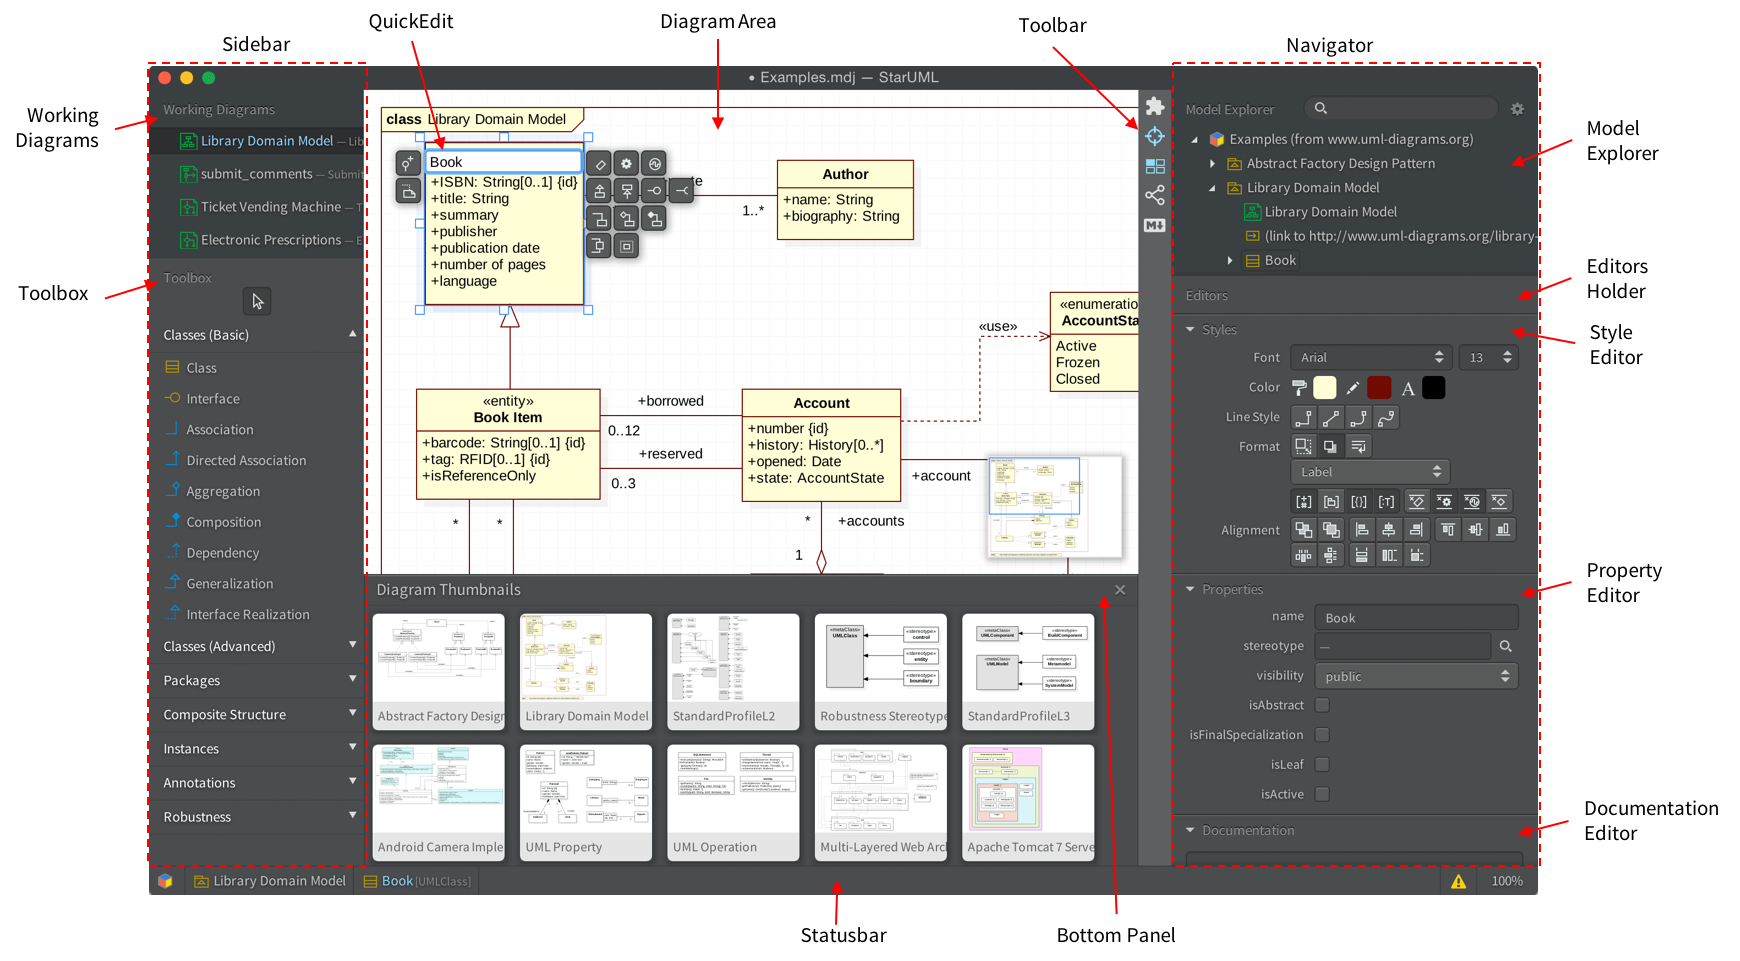
\includegraphics[width=\linewidth]{images/mainwindow}
	\caption{Главное окно}
	\label{fig:mainwindow}
\end{figure}

\sectionunderl{Меню}
Эта секция описывает подробно все пункты в главное меню \staruml TM.StarUNL. Руководство пользователя.
\begin{itemize}
	\item Меню File
	\item Меню Edit
	\item Меню Format
	\item Меню Model
	\item Меню View
	\item Меню Tools
	\item Меню Help
	Горячие клавиши
\end{itemize}
\newpage
\subsubsection*{Меню File}
Меню File содержит следующие пункты меню.
% TODO: \usepackage{graphicx} required
\begin{figure}[h!]
	\centering
	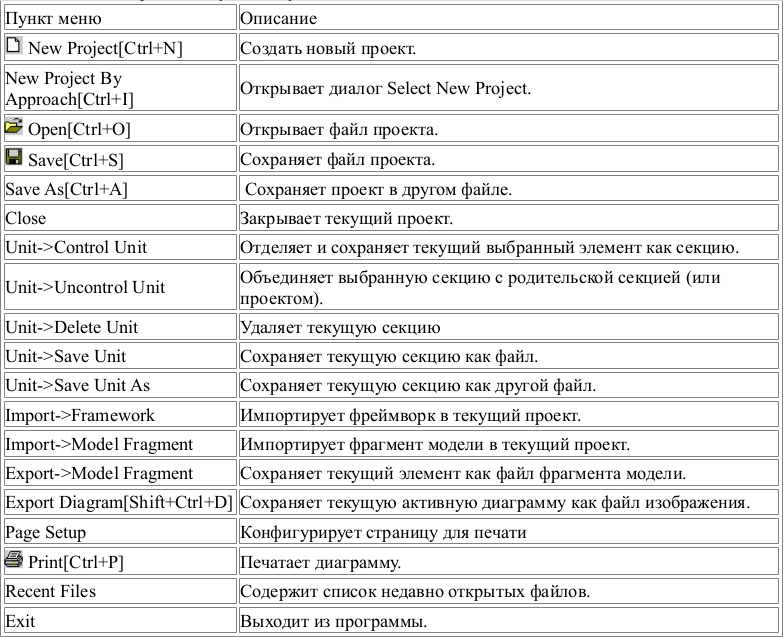
\includegraphics[width=\linewidth]{images/filemenu}
	\caption{Меню File}
	\label{fig:filemenu}
\end{figure}
\newpage
\subsubsection*{Меню Edit}
Меню Edit содержит следующие пункты меню.
% TODO: \usepackage{graphicx} required
\begin{figure}[h!]
	\centering
	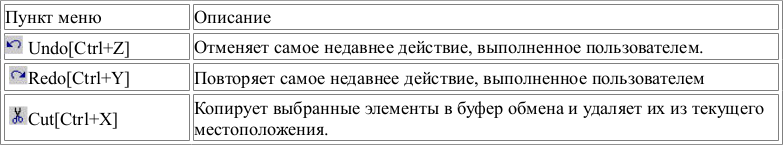
\includegraphics[width=\linewidth]{images/editmenu1}
	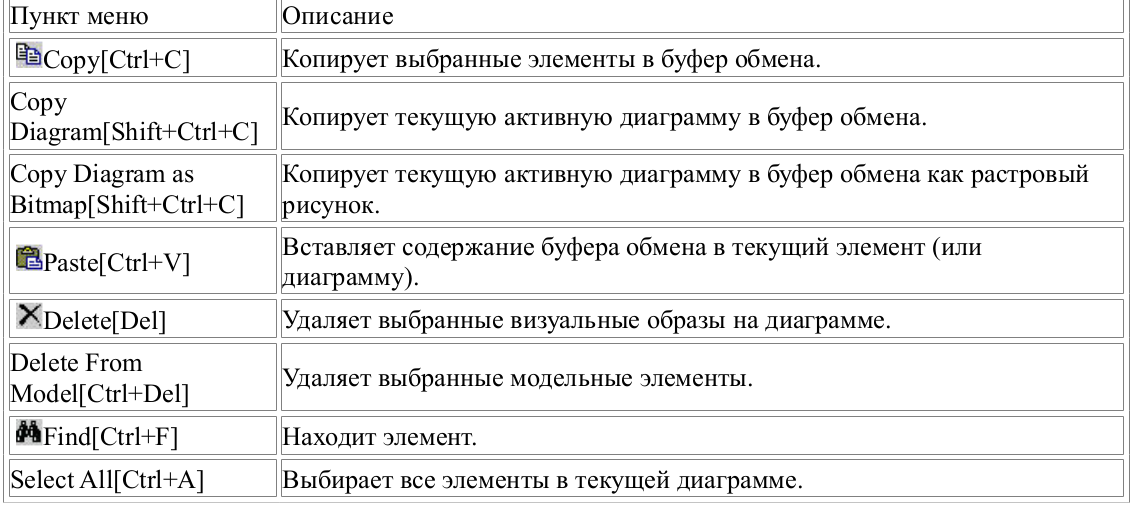
\includegraphics[width=1.005\linewidth]{images/editmenu2}
	\caption{Меню Edit}
	\label{fig:editmenu}
\end{figure}
\newpage
\subsubsection*{Меню Format}
Меню Format содержит следующие пункты меню.
% TODO: \usepackage{graphicx} required
\begin{figure}[h!]
	\centering
	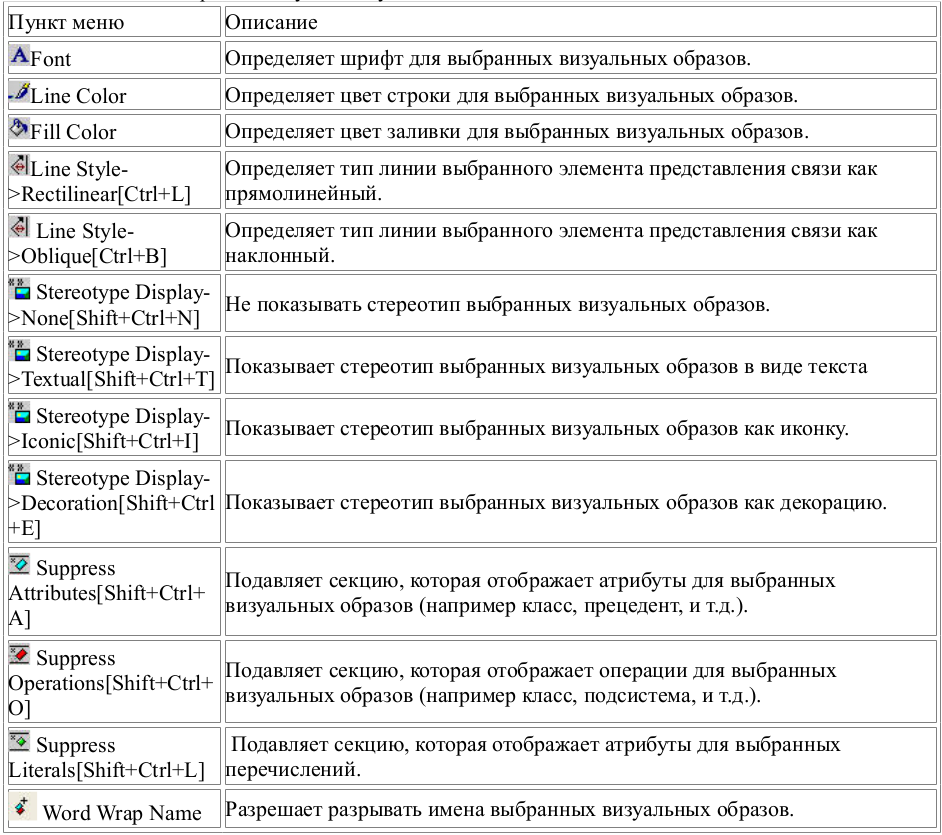
\includegraphics[width=0.7\linewidth]{images/formatmenu1}
	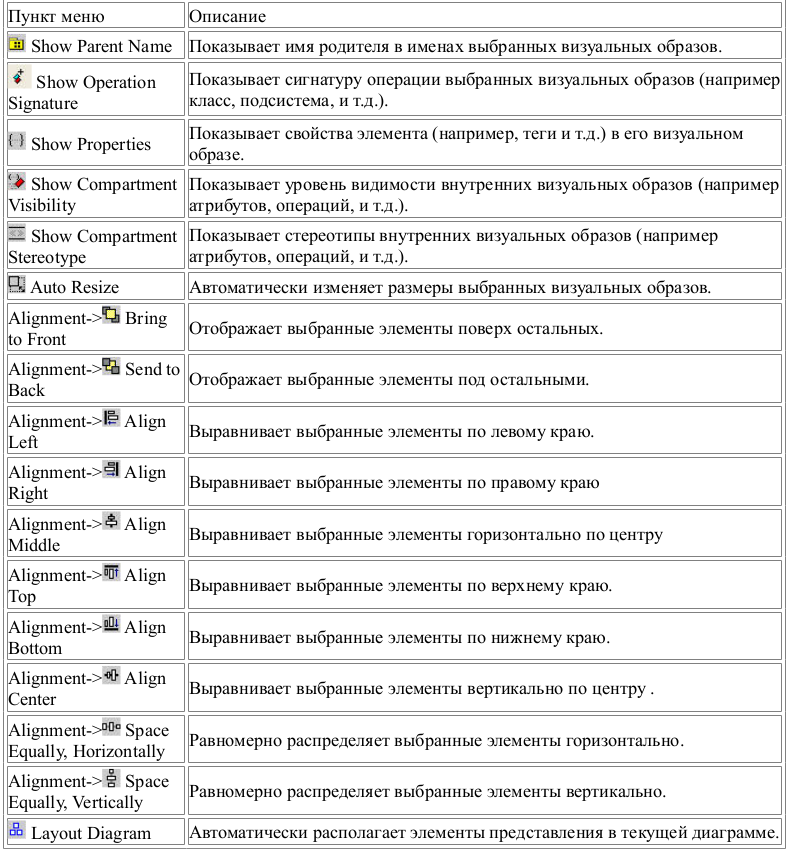
\includegraphics[width=0.7005\linewidth]{images/formatmenu2}
	\caption{Меню Format}
	\label{fig:formatmenu}
\end{figure}

\subsubsection*{Меню View}
Меню Format содержит следующие пункты меню.
% TODO: \usepackage{graphicx} required
\begin{figure}[h!]
	\centering
	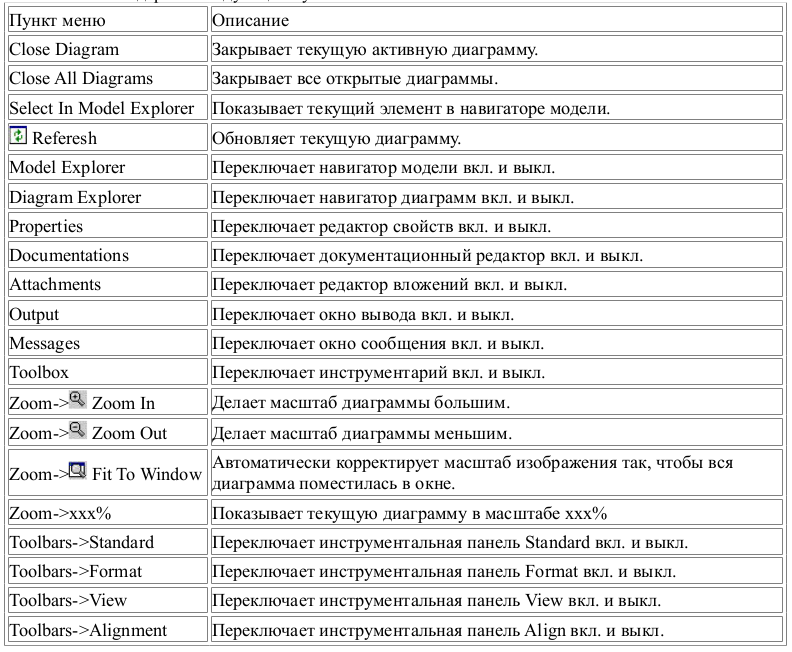
\includegraphics[width=\linewidth]{images/viewmenu}
	\caption{Меню View}
	\label{fig:viewmenu}
\end{figure}


\subsection*{Горячие клавиши}
\staruml обеспечивает горячие клавиши к функциям меню.

\small
\begin{longtable}{|l|l|l|}
			 
			\hline	
			\multicolumn{1}{|c|}{\textbf{Command}} & \multicolumn{1}{c|}{\textbf{MacOS}} & \multicolumn{1}{c|}{\textbf{Windows}} \\ \hline
			\endfirsthead
			
			\multicolumn{3}{c}%
			{{\bfseries \tablename\ \thetable{} -- продолжение}} \\
			
			\hline	
			\multicolumn{1}{|c|}{\textbf{Command}} & \multicolumn{1}{c|}{\textbf{MacOS}} & \multicolumn{1}{c|}{\textbf{Windows}}  \\ \hline
			\endhead
			
			\hline \multicolumn{3}{|r|}{{Продолжение на следующей странице}} \\ \hline
			\endfoot
			
			%\hline \hline
			\endlastfoot
			
			File > New & Cmd+N & Ctrl+N  \\\hline
			File > Open & Cmd+O & Ctrl+O \\ \hline
			File > Save & Cmd+S & Ctrl+S \\ \hline
			File > Save As & Cmd+Shift+S & Ctrl+Shift+S \\ \hline
			File > Preferences & Cmd+, & n/a \\ \hline
			File > Quit & Cmd+Q & Ctrl+Q \\ \hline
			Edit > Undo & Cmd+Z & Ctrl+Z \\ \hline
			Edit > Redo & Cmd+Y & Ctrl+Y \\ \hline
			Edit > Cut & Cmd+X & Ctrl+X \\ \hline
			Edit > Copy & Cmd+C & Ctrl+C \\ \hline
			Edit > Copy Diagram As Image & Cmd+Shift+C & Ctrl+Shift+C \\ \hline
			Edit > Paste & Cmd+V & Ctrl+V \\ \hline
			Edit > Delete & Delete & Delete \\ \hline
			Edit > Delete from Model & Cmd+Delete & Ctrl+Delete \\ \hline
			Edit > Move Up & Cmd+Shift+Up & Ctrl+Shift+Up \\ \hline
			Edit > Move Down & Cmd+Shift+Down & Ctrl+Shift+Down \\ \hline
			Edit > Select All & Cmd+A & Ctrl+A \\ \hline
			Edit > Select In Explorer & Cmd+E & Ctrl+E \\ \hline
			Edit > Select In Diagram & Cmd+D & Ctrl+D \\ \hline
			Format > Font & Cmd+Shift+F & Ctrl+Shift+F \\ \hline
			Format > Fill Color & Cmd+Shift+I & Ctrl+Shift+I \\ \hline
			Format > Line Color & Cmd+Shift+L & Ctrl+Shift+L \\ \hline
			Format > Line Style > Rectilinear & Cmd+L & Ctrl+L \\ \hline
			Format > Line Style > Oblique & Cmd+B & Ctrl+B \\ \hline
			Format > Line Style > RoundRect & Cmd+Option+L & Ctrl+Alt+L \\ \hline
			Format > Line Style > Curve & Cmd+Option+B & Ctrl+Alt+B \\ \hline
			Format > Auto Resize & Cmd+Shift+R & Ctrl+Shift+R \\ \hline
			Format > Show Shadow & Cmd+Shift+H & Ctrl+Shift+H \\ \hline
			Format > Stereotype Display > None & Cmd+Shift+0 & Ctrl+Shift+0 \\ \hline
			Format > Stereotype Display > Label & Cmd+Shift+1 & Ctrl+Shift+1 \\ \hline
			Format > Stereotype Display > Decoration & Cmd+Shift+2 & Ctrl+Shift+2 \\ \hline
			Format > Stereotype Display > Decoration Label & Cmd+Shift+3 & Ctrl+Shift+3 \\ \hline
			Format > Stereotype Display > Icon & Cmd+Shift+4 & Ctrl+Shift+4 \\ \hline
			Format > Stereotype Display > Icon Label & Cmd+Shift+5 & Ctrl+Shift+5 \\ \hline
			Format > Word Wrap & Cmd+Shift+W & Ctrl+Shift+W \\ \hline
			Format > Show Visibility & Cmd+Shift+V & Ctrl+Shift+V \\ \hline
			Format > Show Namespace & Cmd+Shift+N & Ctrl+Shift+N \\ \hline
			Format > Show Property & Cmd+Shift+B & Ctrl+Shift+B \\ \hline
			Format > Show Type & Cmd+Shift+Y & Ctrl+Shift+Y \\ \hline
			Format > Show Multiplicity & Cmd+Shift+M & Ctrl+Shift+M \\ \hline
			Format > Show Operation Signature & Cmd+Shift+G & Ctrl+Shift+G \\ \hline
			Format > Suppress Attributes & Cmd+Shift+A & Ctrl+Shift+A \\ \hline
			Format > Suppress Operations & Cmd+Shift+O & Ctrl+Shift+O \\ \hline
			Format > Suppress Receptions & Cmd+Shift+E & Ctrl+Shift+E \\ \hline
			Format > Suppress Literals & Cmd+Shift+T & Ctrl+Shift+T \\ \hline
			Format > Suppress Columns & Cmd+Shift+U & Ctrl+Shift+U \\ \hline
			Model > Find & Cmd+F & Ctrl+F \\ \hline
			View > Command Palette... & Cmd-Shift-P & Ctrl-Shift-P \\ \hline
			View > Close Diagram & F4 & F4 \\ \hline
			View > Close Other Diagrams & Cmd+F4 & Ctrl+F4 \\ \hline
			View > Close All Diagrams & Shift+F4 & Shift+F4 \\ \hline
			View > Next Diagram & Cmd+Shift+] & Ctrl+Shift+] \\ \hline
			View > Previous Diagram & Cmd+Shift+[ & Ctrl+Shift+[ \\ \hline
			View > Zoom In & Cmd++ & Ctrl++ \\ \hline
			View > Zoom Out & Cmd+- & Ctrl+- \\ \hline
			View > Actual Size & Cmd+0 & Ctrl+0 \\ \hline
			View > Fit To Window & Cmd+Option+1 & Ctrl+Alt+1 \\ \hline
			View > Show Grid & Cmd+G & Ctrl+G \\ \hline
			View > Sidebar & Cmd+1 & Ctrl+1 \\ \hline
			View > Navigator & Cmd+2 & Ctrl+2 \\ \hline
			View > Toolbar & Cmd+3 & Ctrl+3 \\ \hline
			View > Statusbar & Cmd+4 & Ctrl+4 \\ \hline
			View > Toolbox & Cmd+5 & Ctrl+5 \\ \hline
			View > Editors & Cmd+6 & Ctrl+6 \\ \hline
			View > Diagram Thumbnails & Cmd+Option+T & Ctrl+Alt+T \\ \hline
			View > Markdown Documentation & Cmd+Option+D & Ctrl+Alt+D \\ \hline
			View > Minimap & Cmd+Option+M & Ctrl+Alt+M \\ \hline
			View > Relationships & Cmd+Option+R & Ctrl+Alt+R \\ \hline
			Debug > Show DevTools & Shift+Option+T & Shift+Alt+T \\ \hline
			Debug > Reload & Cmd+R & Ctrl+R \\ \hline
\end{longtable}
\normalsize

\sectionunderl{Панели инструментов}
Эта секция описывает все элементы инструментальной панели \staruml TM.
\begin{itemize}
	\item Панель Standard. Включает команды меню File, Edit и Model.
	\item Панель Format. Включает команды меню Format.
	\item Панель View . Включает команды меню View.
	\item Панель Align. Включает команды выравнивания из меню Format.
	\item Панель Pallet. Содержит клавиши для размещения визуальных образов на диаграммах.
\end{itemize}

\subsubsection*{Общие инструменты палитры}
Следующие функции всегда доступны в инструментальной палитре независимо от типов
диаграмм.
% TODO: \usepackage{graphicx} required
\begin{figure}[h!]
	\centering
	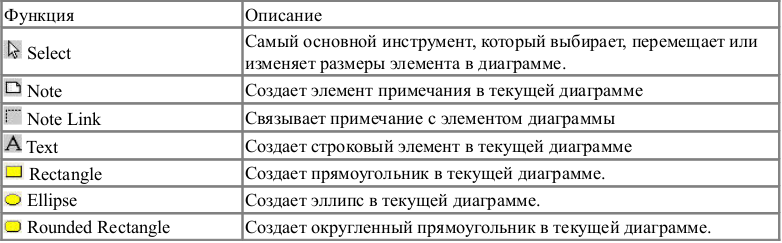
\includegraphics[width=1\linewidth]{images/commoninstruments}
	\caption{Общие инструменты}
	\label{fig:commoninstruments}
\end{figure}


\subsubsection*{Инструменты палитры ориентированные на разные типы диаграмм}
Следующие функции создают элементы для диаграмм разных типов.
% TODO: \usepackage{graphicx} required
\begin{figure}[h!]
	\centering
	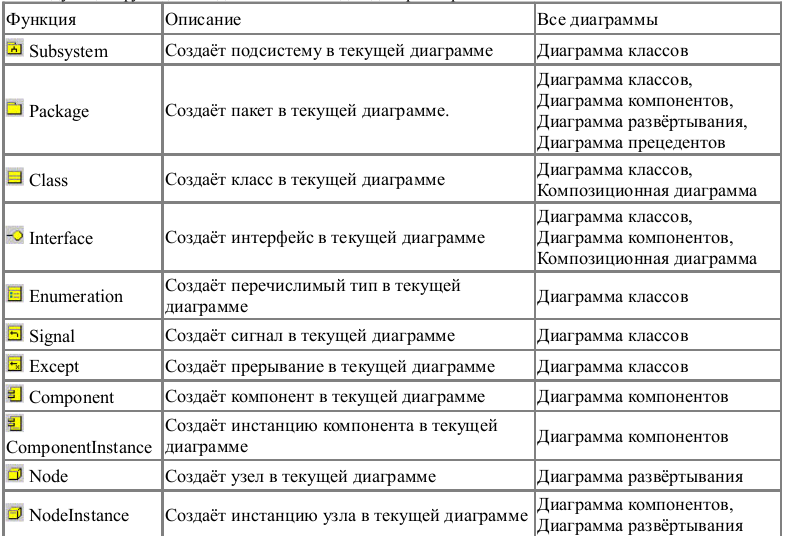
\includegraphics[width=0.9\linewidth]{images/diffinstruments1}
	\caption{Особые инструменты. Ч1}
	\label{fig:diffinstruments1}
\end{figure}
\newpage
% TODO: \usepackage{graphicx} required
\begin{figure}[h!]
	\centering
	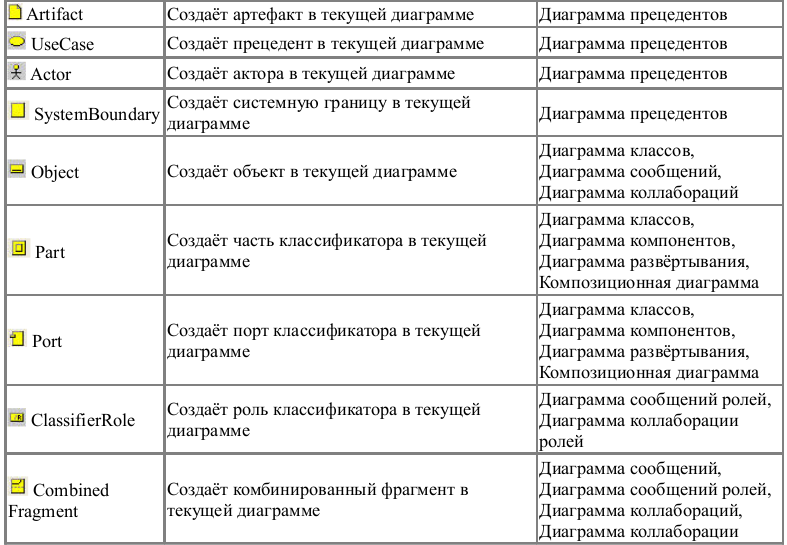
\includegraphics[width=0.9\linewidth]{images/diffinstruments2}
	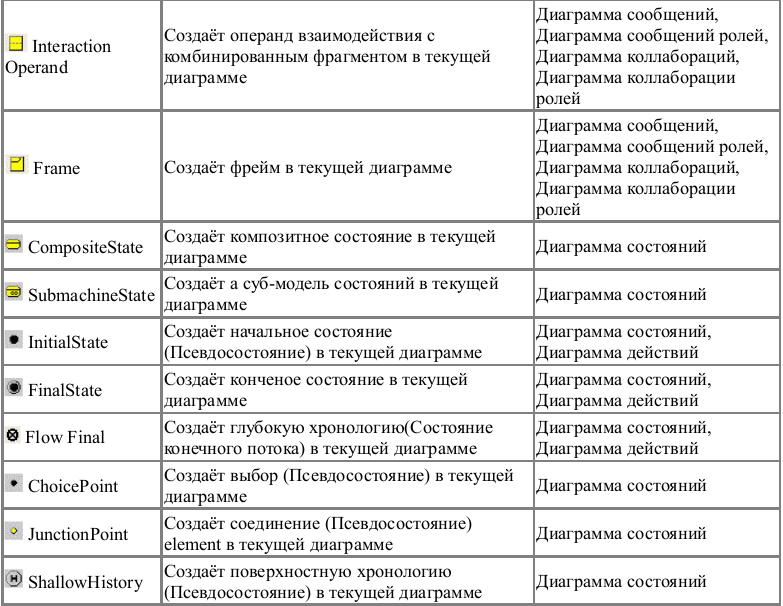
\includegraphics[width=0.9\linewidth]{images/diffinstruments3}
	\caption{Особые инструменты. Ч2}
	\label{fig:diffinstruments2}
\end{figure}
% TODO: \usepackage{graphicx} required
\begin{figure}
	\centering
	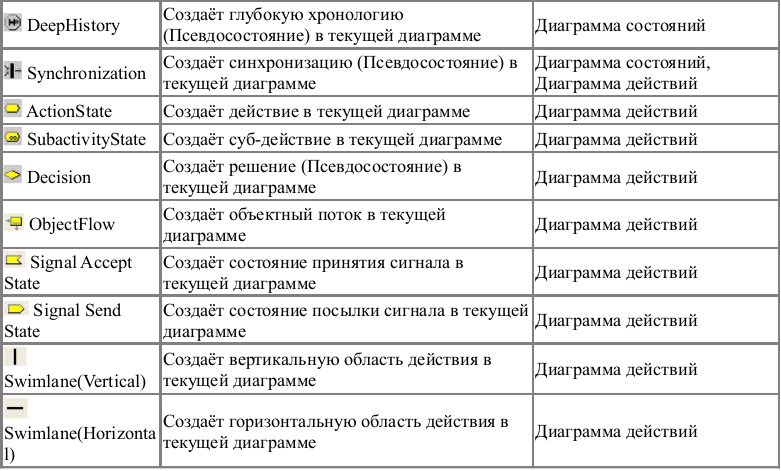
\includegraphics[width=0.9\linewidth]{images/diffinstruments4}
	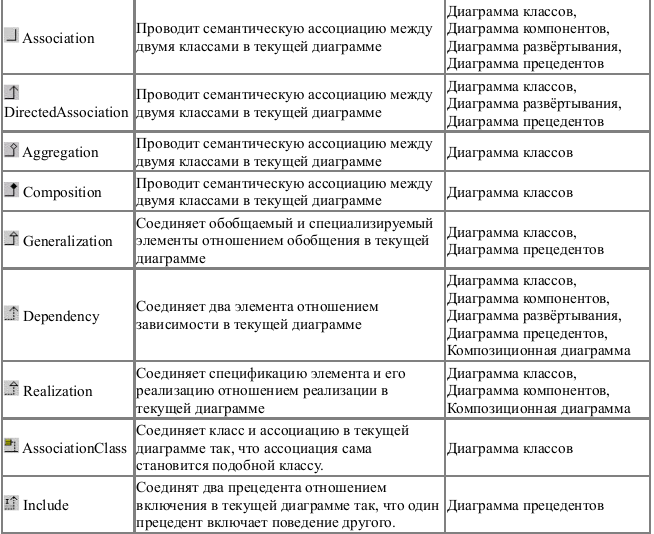
\includegraphics[width=0.9055\linewidth]{images/diffinstruments5}
	\caption{Особые инструменты. Ч3}
	\label{fig:diffinstruments3}
\end{figure}
\begin{figure}
	\centering
	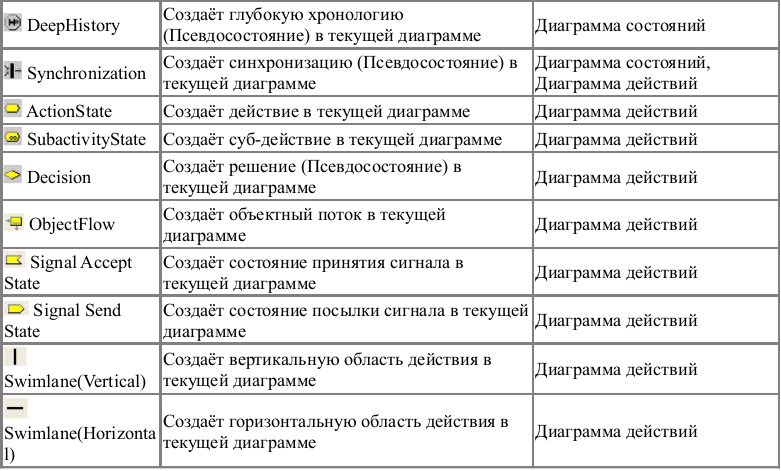
\includegraphics[width=0.9\linewidth]{images/diffinstruments4}
	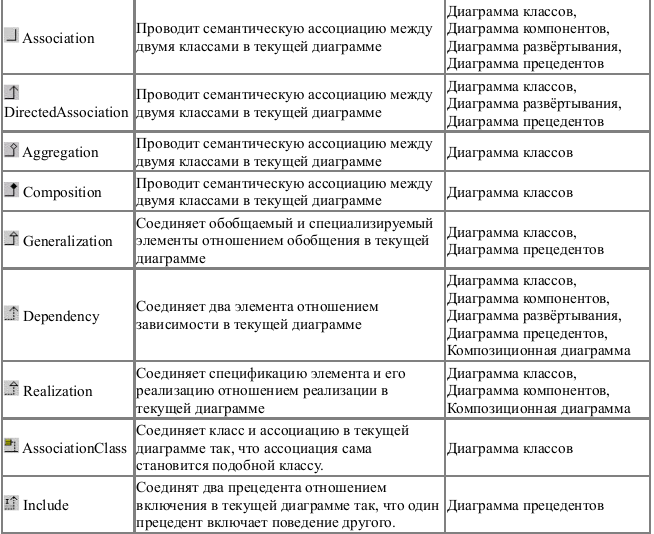
\includegraphics[width=0.9055\linewidth]{images/diffinstruments5}
	\caption{Особые инструменты. Ч4}
	\label{fig:diffinstruments4}
\end{figure}
\newpage
% TODO: \usepackage{graphicx} required
\begin{figure}[h!]
	\centering
	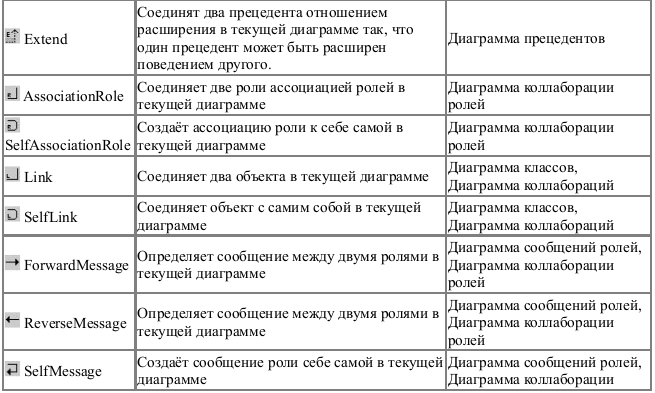
\includegraphics[width=0.9\linewidth]{images/diffinstruments6}
	\caption{Особые инструменты. Ч5}
	\label{fig:diffinstruments5}
\end{figure}


\chapter{Построение диаграмм UML с помощью ПО SrarUML\tm}

\section{Особенности разработки диаграмм вариантов использования (Use Case Diagram)}

Работа над моделью в среде SrarUML\tm начинается с общего
анализа проблемы и построения диаграммы вариантов использования,
которая отражает функциональное назначение проектируемой программной
системы.
В качестве проекта далее будет рассматриваться процесс создания новой модели велосипеда на промышленном предприятии.

Для изменения имени
проекта, предложенного программой по умолчанию, следует сохранить
модель во внешнем файле на диске, например, под именем CycleComp.mdj.
В этом случае изменится имя в строке заголовка и имя проекта в
иерархическом представлении модели в браузере проекта.
Настройка шрифтов, цвета линий и графических элементов
производится или в меню <<Format>>.
В левом нижнем углу в блоке Editors. Характерной особенностью среды является
возможность работы с символами кириллицы. Однако следует заметить,
что при спецификации элементов модели с последующей генерацией
текста программного кода следует записывать имена и свойства
классов, ассоциаций , атрибутов, операций и компонентов символами
того языка, который поддерживается соответствующим языком
программирования.
Для разработки диаграммы вариантов использования модели в среде
\staruml необходимо активизировать соответствующую
диаграмму в окне диаграммы. Это можно сделать следующими способами:
\begin{itemize}
	\item Перейдя в пункт меню $Model \to Add Diagram \to Use Case Diagram$
	
	\item Нажав правой кнопкой мыши на рабочей области и перейдя по $Add Diagram \to Use Case Diagram$
\end{itemize}
При этом появляется новое окно с чистым рабочим листом диаграммы вариантов использования и специальная панель инструментов, содержащая кнопки с изображением графических элементов, необходимых для разработки \textit{диаграммы вариантов использования}. См рис. \ref{fig:toolboxusecase}. Назначение кнопок приведены в таблице \ref{tab:toolboxusecase}.

\subsubsection*{Добавление актера на диаграмму вариантов использования и редактирование его свойств}
Для добавления актера на диаграмму варианта использования нужно с помощью левой кнопки мыши нажать кнопку с изображением пиктограммы актера на специальной панели инструментов, отпустить левую кнопку мыши и щелкнуть левой кнопкой мыши на свободном месте рабочего листа диаграммы. На диаграмме появится изображение актера с маркерами изменения его геометрических размеров и предложенным программой именем по умолчанию \textit{Actor}. Для разрабатываемой модели предложенное программой имя актера следует изменить на \textit{Инженер-конструктор}. См. рис. \ref{fig:actor1}.
% TODO: \usepackage{graphicx} required
% TODO: \usepackage{graphicx} required
\begin{figure}[htbp]
	\centering
	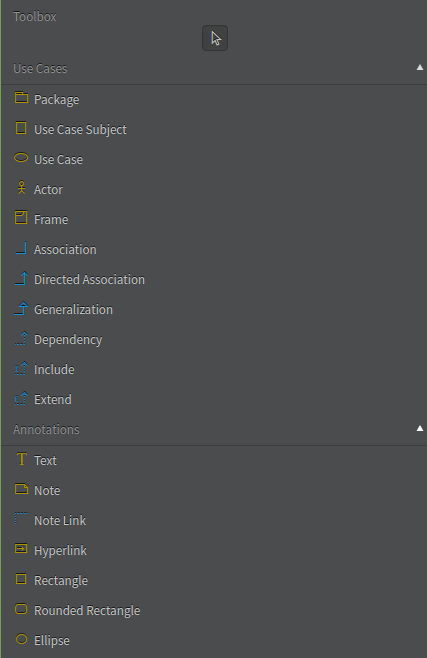
\includegraphics[width=0.4\linewidth]{images/toolboxusecase}
	\caption{Use Case: Панель инструментов}
	\label{fig:toolboxusecase}
\end{figure}
% TODO: \usepackage{graphicx} required
% TODO: \usepackage{graphicx} required
\begin{figure}
	\centering
	
\includegraphics[width=0.3\linewidth]{images/actor1}
	\caption{Use Case:Actor}
	\label{fig:actor1}
\end{figure}


\newpage
\begin{table}[htbp]
	
	\begin{center}
		\begin{tabular}{|l|m{0.5\linewidth}|}
		\hline
		\textbf{Всплывающая подсказка} & \textbf{Назначение кнопки} \\ \hline
		Selection Tool & Превращает изображение курсора в форму стрелки для последующего выделения элементов на диаграмме \\ \hline
		Text Box & Добавляет на диаграмму текстовую область \\ \hline
		Note & Добавляет на диаграмму примечание \\ \hline
		Anchor Note to Item & Добавляет на диаграмму связь примечания с соответствующим графическим элементом диаграммы \\ \hline
		Package & Добавляет на диаграмму пакет \\ \hline
		Use Case & Добавляет на диаграмму вариант использования \\ \hline
		Actor & Добавляет на диаграмму актера \\ \hline
		Unidirectional Association & Добавляет на диаграмму направленную ассоциацию \\ \hline
		Dependency or Instantiates & Добавляет на диаграмму отношение зависимости \\ \hline
		Generalization & Добавляет на диаграмму отношение обобщения \\ \hline
	\end{tabular}
	\end{center}
	\label{tab:toolboxusecase}
	\caption{Use Case: Назначение кнопок}
\end{table}
Чтобы изменить графические размеры изображения элемента модели, прежде всего, следует щелчком левой кнопки мыши выделить его в рабочей области диаграммы.

Имя размещенного на диаграмму элемента разработчик может изменить либо сразу после добавления элемента на диаграмму, либо в ходе последующей работы над проектом. Для любого графического элемента модели по щелчку правой кнопкой мыши на выбранном элементе вызывается контекстное меню данного элемента. Подробнее ознакомиться с параметрами выбранного элемента можно в области \textit{Editors}, расположенной справа от рабочей области. Для добавленного актера \textit{<<Инженер-конструктор>>} окно спецификации свойств выглядит следующим образом. См рис. \ref{fig:actor1editors}.

\newpage
% TODO: \usepackage{graphicx} required
\begin{figure}[htbp]
	\centering
	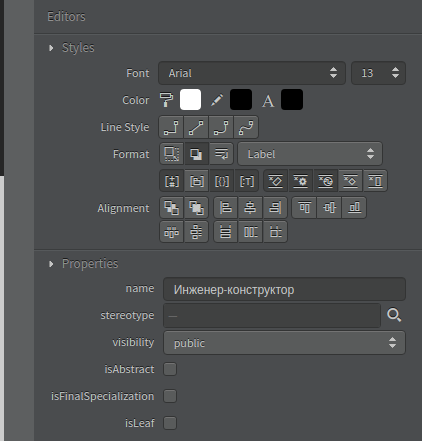
\includegraphics[width=0.5\linewidth]{images/actor1editors}
	\caption{Спецификация актера}
	\label{fig:actor1editors}
\end{figure}

В среде \staruml актер является классом, для него некорректно специфицировать атрибуты и операции, поскольку актер является внешней по отношению к разрабатываемой системе сущностью.
Для актера \textit{Инженер-конструктор} можно уточнить его назначение в модели. С этой целью следует изменить его стереотип и добавить текст документации. Для добавления текста документации в секцию Documentation следует ввести текст: <<Физическое лицо, осуществляющее инженерную деятельность>> и нажать кнопку Apply (Применить) или OK. После изменения данных свойств актера \textit{Инженер-конструктор} окно спецификации свойств будет выглядеть следующим образом \ref{fig:actor1editors2}.

\subsubsection{Добавление и редактирование варианта использования}
Для добавления варианта использования на диаграмму нужно с помощью левой кнопки мыши нажать кнопку с изображением варианта использования на специальной панели инструментов, отпустить левую кнопку мыши и щелкнуть левой кнопкой мыши на свободном месте диаграммы. На диаграмме появится изображение варианта использования с маркерами изменения его геометрических размеров и предложенным программой именем по умолчанию \textit{UseCase}. Для разрабатываемой модели предприятия предложенное программой имя варианта использования следует изменить на \textit{Спроектировать изделие} (рис. \ref{fig:usecaseproectdaction}).
\newpage
% TODO: \usepackage{graphicx} required
\begin{figure}[h!]
	\centering
	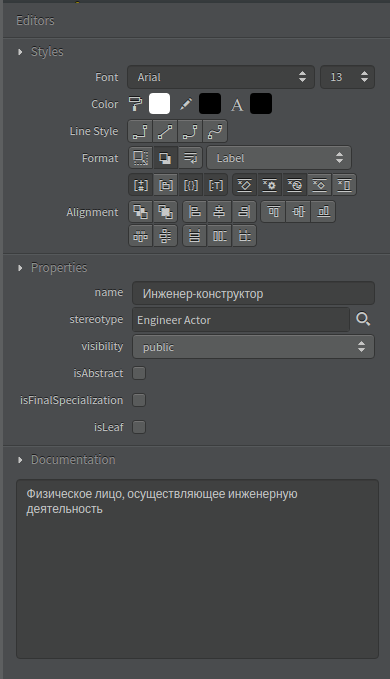
\includegraphics[width=0.35\linewidth]{images/actor1editors2}
	\caption{Измененная спецификация актера}
	\label{fig:actor1editors2}
\end{figure}

% TODO: \usepackage{graphicx} required
\begin{figure}[h!]
	\centering
	
\includegraphics[width=0.8\linewidth]{images/usecaseproectdaction}
	\caption{Вариант использования}
	\label{fig:usecaseproectdaction}
\end{figure}

Для уточнения свойств данного варианта использования следует открыть диалоговое окно спецификации его свойств, например, с помощью двойного щелчка левой кнопкой мыши на изображении этого элемента на диаграмме. Для изменения стереотипа во вложенном списке Stereotype нужно выбрать строку Engineer Use Case. Для добавления текста документации в секцию Documentation следует ввести текст: "Основной вариант использования для разрабатываемой модели предприятия" и нажать кнопку Apply (Применить) или OK. После изменения данных свойств варианта использования окно спецификации его свойств будет выглядеть следующим образом (рис. \ref{fig:actioneditors}).


% TODO: \usepackage{graphicx} required
\begin{figure}[h!]
	\centering
	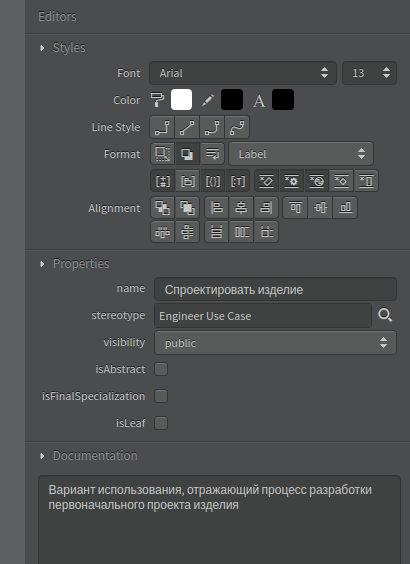
\includegraphics[width=0.4\linewidth]{images/actioneditors}
	\caption{Дополненная спецификация варианта использования}
	\label{fig:actioneditors}
\end{figure}


\subsubsection*{Добавление ассоциации}
Для добавления ассоциации между актером и вариантом использования на диаграмму нужно с помощью левой кнопки мыши нажать на специальной панели инструментов кнопку с изображением пиктограммы направленной ассоциации, отпустить левую кнопку мыши, щелкнуть левой кнопкой мыши на изображении актера на диаграмме и отпустить ее на изображении варианта использования. В результате этих действий на диаграмме появится изображение ассоциации, соединяющей актера с вариантом использования. См. рис. \ref{fig:actorwithaction}.
%\newpage
% TODO: \usepackage{graphicx} required
\begin{figure}[h!]
	\centering
	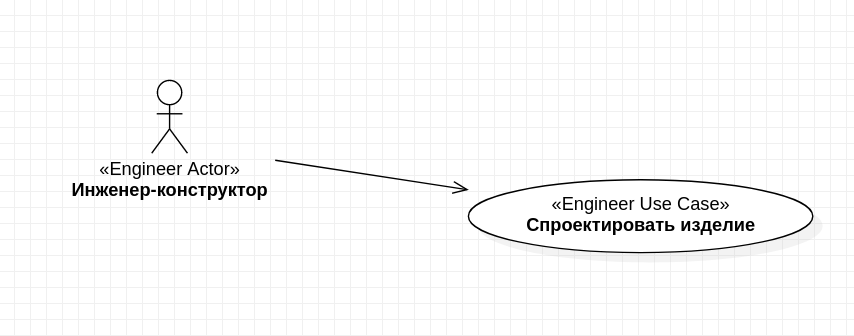
\includegraphics[width=0.8\linewidth]{images/actorwithaction}
	\caption{Ассоциация актера с вариантом использования}
	\label{fig:actorwithaction}
\end{figure}
При необходимости можно сделать направленную ассоциацию ненаправленной, для чего следует воспользоваться секцией \textit{Editors}, расположенной справа, под Обозревателем Модели (\textit{Model Explorer}). Следует убрать отметку строки выбора \textit{Navigable} (Навигация) (рис. \ref{fig:navigable}).
\newpage

% TODO: \usepackage{graphicx} required
\begin{figure}[h!]
	\centering
	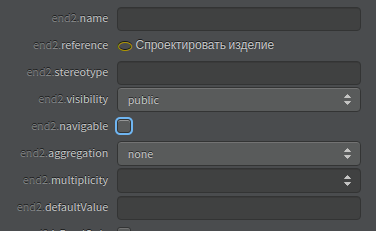
\includegraphics[width=0.5\linewidth]{images/navigable}
	\caption{Свойство Navigable}
	\label{fig:navigable}
\end{figure}


\subsubsection*{Добавление отношения зависимости и редактирование его свойств}
Для добавления отношения зависимости между двумя вариантами использования на диаграмму необходимо предварительно рассмотренным выше способом добавить второй вариант использования с именем \textit{Изготовить тестовый образец}. После этого с помощью левой кнопки мыши нажать кнопку с изображением пиктограммы зависимости на специальной панели инструментов, отпустить левую кнопку мыши, щелкнуть левой кнопкой мыши на изображении варианта использования \textit{Спроектировать изделие} и отпустить ее на изображении варианта использования \textit{Изготовить тестовый образец}. 

В результате этих действий на диаграмме появится изображение отношения зависимости, которое соединяет два выбранных варианта использования.
Поскольку вариант использования \textit{Спроектировать изделие} выполняется всегда, для добавленного отношения зависимости дополнительно следует указать текстовый стереотип <<include>>. Выполнить это можно уже известным способом с помощью диалогового окна спецификации свойств этого отношения и выбора нужного стереотипа из предлагаемого списка.

После задания для данного отношения зависимости стереотипа <<include>> текст этого стереотипа в угловых скобках появится рядом с изображением пунктирной линии зависимости, связывающей соответствующие варианты использования (рис. \ref{fig:actionsinclude}). С целью лучшей визуализации диаграммы текстовую область стереотипа можно переместить в нужное место диаграммы. Выполнить это можно с помощью общего способа перемещения графических элементов модели, который был рассмотрен ранее применительно к актеру \textit{Инженер-конструктор}.
\newpage
% TODO: \usepackage{graphicx} required
\begin{figure}[h!]
	\centering
	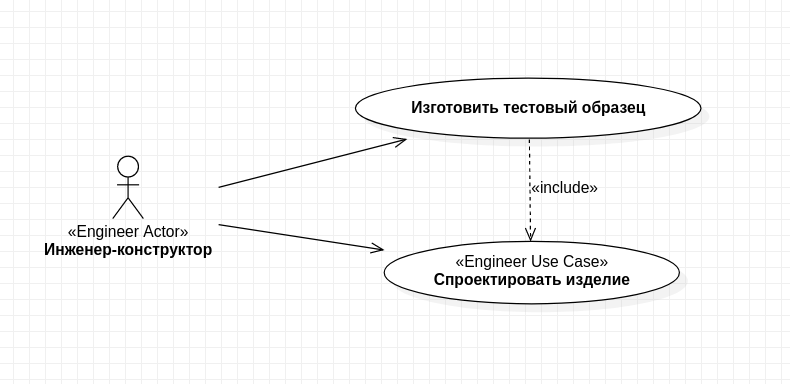
\includegraphics[width=0.7\linewidth]{images/actionsinclude}
	\caption{Отношение зависимости между вариантами использования}
	\label{fig:actionsinclude}
\end{figure}
Аналогичным образом могут быть добавлены на диаграмму вариантов использования отношения зависимости со стереотипом <<extend>>, которые применяются для моделирования исключений при выполнении отдельных вариантов использования.

\subsubsection*{Удалеие графического элемента}
Для удаления любого графического элемента с диаграммы его следует выделить на диаграмме и нажать клавишу \textit{Delete} на клавиатуре. При этом выделенный элемент будет удален с активной диаграммы, но не из модели. Для удаления элемента не только из диаграммы, но и из модели проекта необходимо выбрать пункт \textit{Delete From Model} в диалоговом окне, появляющимся при попытке удаления объекта. 

\subsubsection*{Построение диаграммы}
Завершим построение \textit{Диаграммы Вариантов использования}, добавив необходимых актеров и соответствующие варианты использования. См. рис. \ref{fig:usecase}.
% TODO: \usepackage{graphicx} required
\newpage
\begin{figure}[h!]
	\centering
	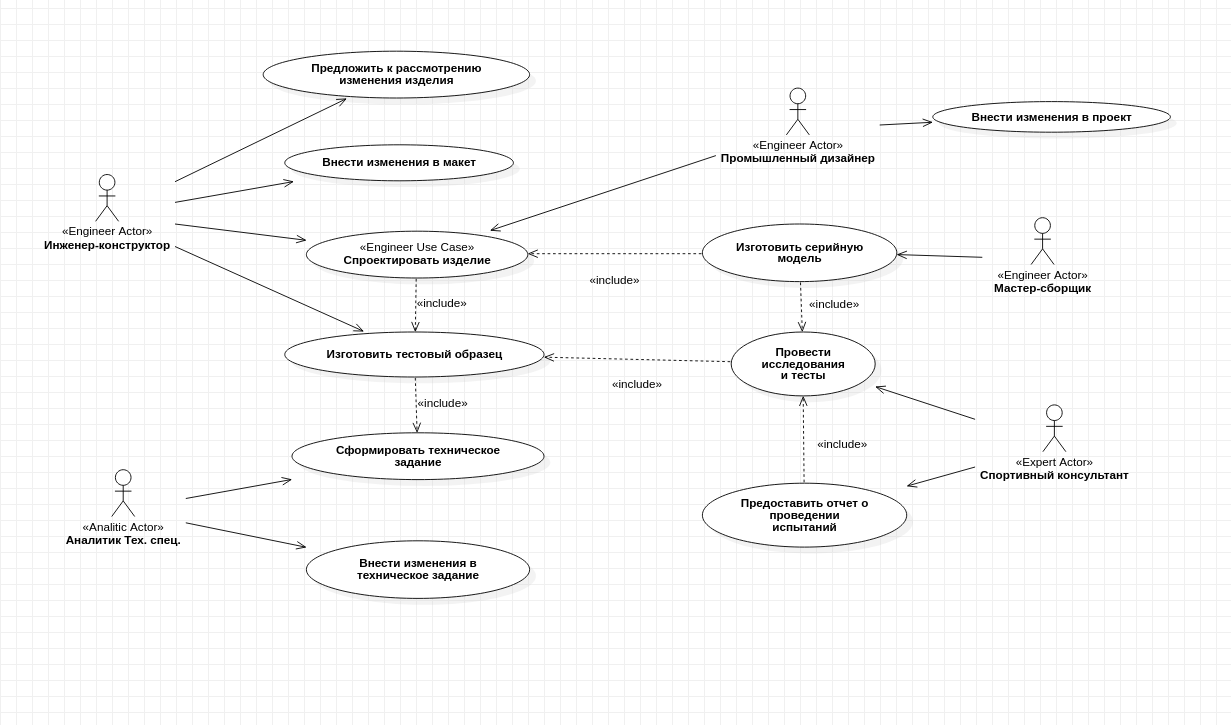
\includegraphics[width=\linewidth]{images/usecase}
	\caption{Диаграмма вариантов использования}
	\label{fig:usecase}
\end{figure}

Напомним, что диаграмма вариантов использования является высокоуровневым концептуальным представлением модели, поэтому она не должна содержать слишком много вариантов использования и актеров. В последующем построенная диаграмма может быть изменена посредством добавления новых элементов, таких как варианты использования и актеры, или их удаления.

При работе с отношениями на диаграмме вариантов использования следует помнить о назначении соответствующих отношений в нотации языка UML. Речь идет о том, что если для двух элементов выбранный вид отношения не является допустимым, то в большинстве случаев программа \staruml сообщит об этом разработчику, и соответствующая линия связи не будет добавлена на диаграмму.
После окончания сеанса работы над проектом выполненную работу необходимо сохранить в файле проекта с расширением <<.mdj>>. 


\section{Особенности разработки диаграмм классов (Class Diagram)}
Диаграмма классов является основным логическим представлением модели и содержит детальную информацию о внутреннем устройстве объектно-ориентированной программной системы или, используя современную терминологию, об архитектуре программной системы. Активизировать рабочее окно диаграммы классов можно несколькими способами:
\begin{itemize}
	\item окно диаграммы классов появляется по умолчанию в рабочем окне диаграммы после создания нового проекта;
	\item выбрать соответствующий вариант, перейдя по следующим пунктам меню: \\$Model \to Add Diagram \to Class Diagram$;
	\item нажать правую кнопку мыши на рабочей области и выбрать аналогичные пункты контекстного меню: $Add Diagram \to Class Diagram$;
\end{itemize}

При этом появляется новое окно с чистым рабочим листом диаграммы классов и специальная панель инструментов, содержащая кнопки с изображением графических примитивов, необходимых для разработки диаграммы классов (рис. \ref{fig:toolboxclass}). Назначение отдельных кнопок панели можно узнать также из всплывающих подсказок. Приведем назначение некоторых инструментов в таблице \ref{tab:toolboxclass}.

% TODO: \usepackage{graphicx} required
\begin{figure}[h!]
	\centering
	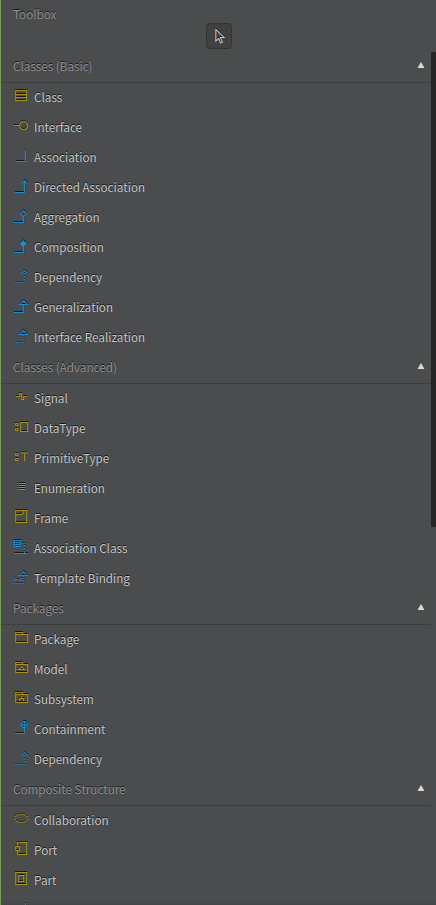
\includegraphics[width=0.4\linewidth]{images/toolboxclass}
	\caption{Сlass Diagram:Панель инструментов}
	\label{fig:toolboxclass}
\end{figure}


\begin{table}[htbp]
	
	\begin{center}
		\begin{tabular}{|l|m{0.6\linewidth}|}
			\hline
			\textbf{Всплывающая подсказка} & \textbf{Назначение кнопки} \\ \hline
			Selection Tool & Превращает изображение курсора в форму стрелки для последующего выделения элементов на диаграмме \\ \hline
			Text Box & Добавляет на диаграмму текстовую область \\ \hline
			Note & Добавляет на диаграмму примечание \\ \hline
			Anchor Note to Item & Добавляет на диаграмму связь примечания с соответствующим графическим элементом диаграммы \\ \hline
			Class & Добавляет на диаграмму класс \\ \hline
			Interface & Добавляет на диаграмму интерфейс \\ \hline
			Unidirectional Association & Добавляет на диаграмму направленную ассоциацию \\ \hline
			Association Class & Добавляет на диаграмму ассоциацию класс \\ \hline
			Package & Добавляет на диаграмму пакет \\ \hline
			Dependency or Instantiates & Добавляет на диаграмму отношение зависимости \\ \hline
			Generalization & Добавляет на диаграмму отношение обобщения \\ \hline
			Realize & Добавляет на диаграмму отношение реализации \\ \hline
		\end{tabular}
	\end{center}
	\caption{Class Diagram: Назначение пунктов меню}
	\label{tab:toolboxclass}
\end{table}
\subsubsection*{Добавление класса на диаграмму классов и редактирование его свойств}
Для добавления класса на диаграмму классов нужно с помощью левой кнопки мыши нажать кнопку с изображением пиктограммы класса на специальной панели инструментов, отпустить левую кнопку мыши и щелкнуть левой кнопкой мыши на свободном месте рабочего листа диаграммы. На диаграмме появится изображение класса с маркерами изменения его геометрических размеров и предложенным средой именем по умолчанию \textit{Class}.

Продолжая разработку модели предприятия по производству велосипедов в качестве сквозного примера проекта, построим для этой модели следующую каноническую диаграмму --- диаграмму классов. С этой целью следует изменить предложенное по умолчанию имя диаграммы Main на ClassDiagramCycle, а имя добавленного на диаграмму класса - на \textit{Конструкторский отдел} \ref{fig:constructclass}.

% TODO: \usepackage{graphicx} required
\begin{figure}[h!]
	\centering
	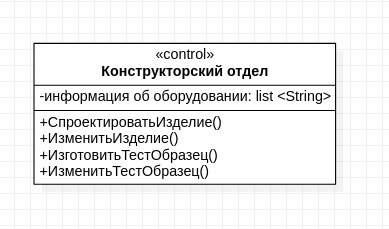
\includegraphics[width=0.7\linewidth]{images/constructclass}
	\caption{Класс <<Конструкторский отдел>>}
	\label{fig:constructclass}
\end{figure}


Поскольку разрабатываемая модель предприятия на начальных этапах работы над проектом используется для анализа общей архитектуры проекта и согласования ее с различными участниками рабочей группы, имена классов, их атрибутов и операций для большей наглядности и понимания задаются на русском языке с пробелами и записываются символами кириллицы.

В последующем по мере выполнения проекта и реализации модели на некотором языке программирования, имена соответствующих классов, атрибутов и операций должны быть преобразованы в символы латиницы. При этом имена этих элементов модели должны быть записаны без пробелов. В контексте управляемой моделью архитектуры первую модель еще называют независимой от платформы реализации, а вторую --- зависимой от платформы реализации.

Для класса \textit{Конструкторский отдел} можно уточнить его назначение в модели с помощью указания стереотипа и пояснительного текста в форме документации. С этой целью щелчком левой кнопкой мыши на изображении этого класса на диаграмме или в браузере проекта открыть секцию \textit{Editors} этого класса и в разделе \textit{Properties} в строке \textit{stereotype} указать стереотип <<control>>. При этом стереотип отобразится над именем класса в угловых кавычках (рис. \ref{fig:classeditors}).

% TODO: \usepackage{graphicx} required
\begin{figure}[h!]
	\centering
	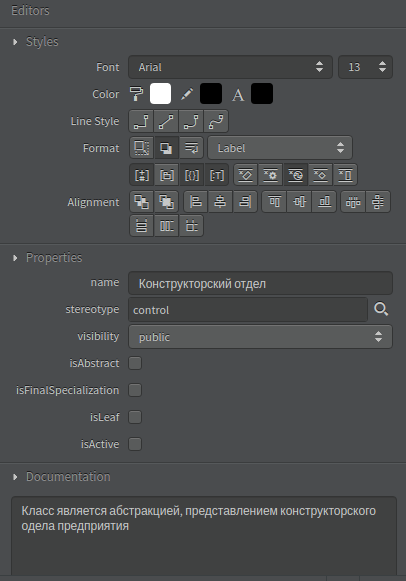
\includegraphics[width=0.5\linewidth]{images/classeditors}
	\caption{Секция Editors}
	\label{fig:classeditors}
\end{figure}



Выбор данного стереотипа означает, что соответствующий класс предназначен для проведения каких-либо процессов, изменяющих состояние сущностей. Данный класс также отвечает за координацию действий других классов.

Далее в секцию документации данного класса можно ввести поясняющий текст: <<Класс является абстракцией, представлением конструкторского одела предприятия>> и нажать кнопку \textit{Apply} или \textit{OK}, чтобы сохранить результаты редактирования свойств выбранного класса.



В разделе \textit{Properties} секции \textit{Editors} можно настроить дополнительные характеристики класса:
\begin{itemize}
	\item Настроить видимость класса характеристикой \textit{visibility} (public, private, protected, package);
	\item Указать класс как абстрактный \textit{(isAbstract)};
	\item Указать реализацию класса как финальную \textit{(isLeaf)};
	\item Указать класс активным \textit{(isActive)}.
\end{itemize}

В той же секции, кликнув на метод конкретного класса можно специфицировать условия на возможность реализации объектов класса в параллельных потоках управления. Для выбора могут быть использованы следующие свойства:
\begin{itemize}
	\item Sequential (Последовательный) --- свойство по умолчанию, которое означает, что объекты класса будут вести себя нормально только при наличии одного потока управления, т. е. соответствующие операции объектов должны выполняться последовательно. В то же время при наличии нескольких потоков управления стабильное поведение объектов класса не гарантируется.
	\item Guarded (Безопасный) --- означает, что при наличии нескольких потоков управления объекты класса будут вести себя ожидаемым от них образом. Для этого объекты в различных потоках должны взаимодействовать друг с другом для того, чтобы гарантировать отсутствие конфликта между ними.
	\item Concurent (Параллельный) --- означает, что объекты класса будут вести себя ожидаемым от них образом при наличии нескольких потоков управления. При этом нет необходимости во взаимодействии объектов в различных потоках управления, поскольку объекты данного класса могут  самостоятельно разрешать возможные конфликты.
\end{itemize}
Продолжая разработку модели предприятия, добавим на диаграмму второй класс с именем \textit{Управляющий отдел}, для которого в окне спецификации свойств выберем стереотип \textit{<<boundary>>} (граничный класс), а в качестве документации введем текст: <<Реализует поведение аналитического отдела. Инициирует работу над новым изделием и вводит изделие в модельный ряд>>.


\subsubsection*{Добавление ассоциации на диаграмму классов и редактирование ее свойств}
Добавление на диаграмму ассоциации между двумя классами выполняется следующим образом. На специальной панели инструментов необходимо нажать кнопку с изображением пиктограммы направленной ассоциации и отпустить левую кнопку мыши. Если ассоциация направленная, то на диаграмме классов надо выделить первый элемент ассоциации или источник, от которого исходит стрелка, и, не отпуская нажатую левую кнопку мыши, переместить ее указатель ко второму элементу отношения или приемнику, к которому направлена стрелка.

После перемещения ко второму элементу кнопку мыши следует отпустить, в результате чего на диаграмму классов будет добавлена направленная ассоциация между двумя выбранными классами.
Продолжая разработку диаграммы классов модели предприятия, добавим на нее описанным способом направленную ассоциацию между классами \textit{Управляющий отдел} и \textit{Конструкторский отдел}).

% TODO: \usepackage{graphicx} required
\begin{figure}[h!]
	\centering
	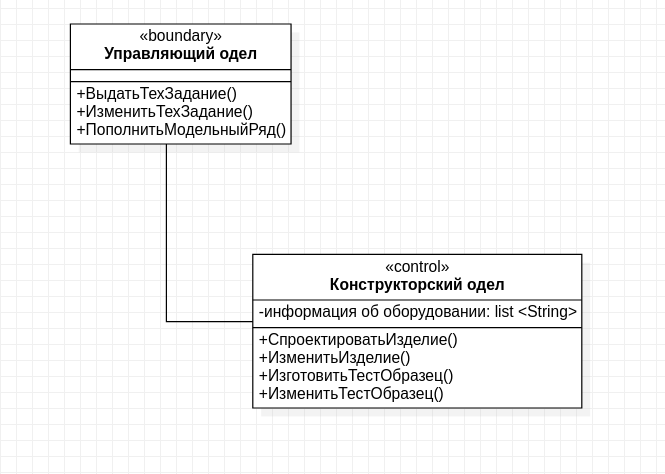
\includegraphics[width=0.7\linewidth]{images/association}
	\caption{Ассоциация}
	\label{fig:association}
\end{figure}

Укажем имя для данной связи. Это можно выполнить с помощью окна спецификации свойств ассоциации. Доступ к секции \textit{Editors} можно получить после выделения линии ассоциации на диаграмме классов или в обозревателе проекта и двойного щелчка левой кнопкой мыши.

Для отдельного класса можно уточнить также и другие его свойства, доступные для редактирования на вкладке \textit{Editors} окна спецификации свойств этого класса. Например, на этой вкладке с помощью атрибута \textit{Multiplicity }(Кратность) можно задать количество объектов или экземпляров данного класса. В данном случае для классов \textit{Конструкторский отдел} и \textit{Управляющий отдел}, связанных ассоциацией, укажем кратность <<один ко многим>> (рис. \ref{fig:associationclasses}). Данная кратность указывает на то, что в ведении аналитического отдела может находиться один или более конструкторских отделов. Но при этом каждый конструкторский отдел получает задания только от одного аналитического отдела. 
% TODO: \usepackage{graphicx} required
\begin{figure}[h!]
	\centering
	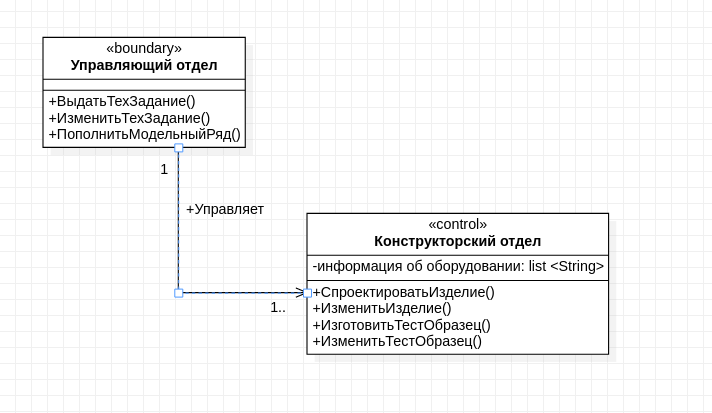
\includegraphics[width=0.7\linewidth]{images/associationclasses}
	\caption{Кратность ассоциации}
	\label{fig:associationclasses}
\end{figure}



\subsubsection*{Добавление отношения обобщения на диаграмму классов и редактирование ее свойств}
Добавление на диаграмму отношения обобщения между двумя классами выполняется следующим образом. На специальной панели инструментов необходимо нажать кнопку с изображением пиктограммы обобщения и отпустить левую кнопку мыши. 

Далее на диаграмме классов надо выделить первый элемент обобщения или потомок, от которого исходит стрелка, и, не отпуская нажатую левую кнопку мыши, переместить ее указатель ко второму элементу отношения или предку, к которому направлена стрелка. После перемещения ко второму элементу кнопку мыши следует отпустить, в результате чего на диаграмму классов будет добавлена линия обобщения между двумя выбранными классами.

Продолжая разработку модели предприятия, добавим на диаграмму третий, абстрактный класс с именем \textit{Отдел}, который будет являться родительским для всех классов, соответственно добавим на диаграмму связи обобщения \textit{(Generalization)}. 

Добавим в описание класса следующие закрытые (private) атрибуты:
\begin{itemize}
	\item Номер отдела: Int
	\item Количество сотрудников: Int
	\item Руководитель отдела: String
\end{itemize}

Последний класс может быть предназначен для спецификации системных атрибутов и операций, необходимых при исполнении соответствующей программы. Напомним, что на абстрактный характер класса указывает написание курсивом его имени, а для спецификации данного свойства класса необходимо на вкладке \textit{Properties} окна спецификации свойств класса \textit{Отел} выставить отметку в строке выбора \textit{isAbstract} (рис. \ref{fig:department}).

% TODO: \usepackage{graphicx} required
\begin{figure}
	\centering
	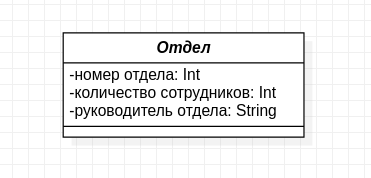
\includegraphics[width=0.7\linewidth]{images/department}
	\caption{Абстрактный класс}
	\label{fig:department}
\end{figure}

 
 
\subsubsection*{Добавление и редактирование атрибутов классов}
Из всех графических элементов среды \staruml класс обладает максимальным набором свойств, главными из которых являются его атрибуты и операции, поскольку именно диаграмма классов используется для генерации программного кода.
Добавить атрибут к созданному ранее классу можно одним из следующих способов:
\begin{itemize}
	\item С помощью операции контекстного меню \textit{Add Attribute} (Добавить атрибут) или воспользоваться сочетанием клавиш \texttt{(Ctrl+Enter)} для класса, выделенного на диаграмме классов. В этом случае активизируется курсор ввода текста в области графического изображения класса на диаграмме;
	\item С помощью операции контекстного меню: $Add \to Atribute$ для класса, нажав правой кнопкой мыши на графическое изображение класса;
	\item Нажав правой копкой мыши на названии класса в секции \textit{Model Explorer} и выбрав пункты контекстного меню: $Add \to Atribute$.
\end{itemize}


\subsubsection*{Добавление и редактирование операций классов}
Функционирование предприятия основано на выполнении его отделами тех или иных действий (процессов). В модели структуры предприятия все действия представляются с помощью операций классов. Таким образом, следующий этап разработки диаграммы классов связан со спецификацией операций классов.

Добавить операцию к созданному ранее классу можно одним из следующих способов:
\begin{itemize}
	\item С помощью операции контекстного меню \textit{Add Operation} (Добавить метод) или воспользоваться сочетанием клавиш \texttt{(Ctrl+Sift+Enter)} для класса, выделенного на диаграмме классов. В этом случае активизируется курсор ввода текста в области графического изображения класса на диаграмме;
	\item С помощью операции контекстного меню: $Add \to Operation$ для класса, нажав правой кнопкой мыши на графическое изображение класса;
	\item Нажав правой копкой мыши на названии класса в секции \textit{Model Explorer} и выбрав пункты контекстного меню: $Add \to Operation$.
\end{itemize}

\subsubsection*{Окончательное построение диаграммы классов модели предприятия}
Для окончательного построения диаграммы классов рассматриваемой модели предприятия следует описанным выше способом добавить оставшиеся классы и ассоциации, а также специфицировать стереотипы, атрибуты и операции этих классов. 

Построенная в результате указанных действий диаграмма классов будет иметь следующий вид (рис. \ref{fig:classdiagram}).

% TODO: \usepackage{graphicx} required
\begin{figure}[h!]
	\centering
	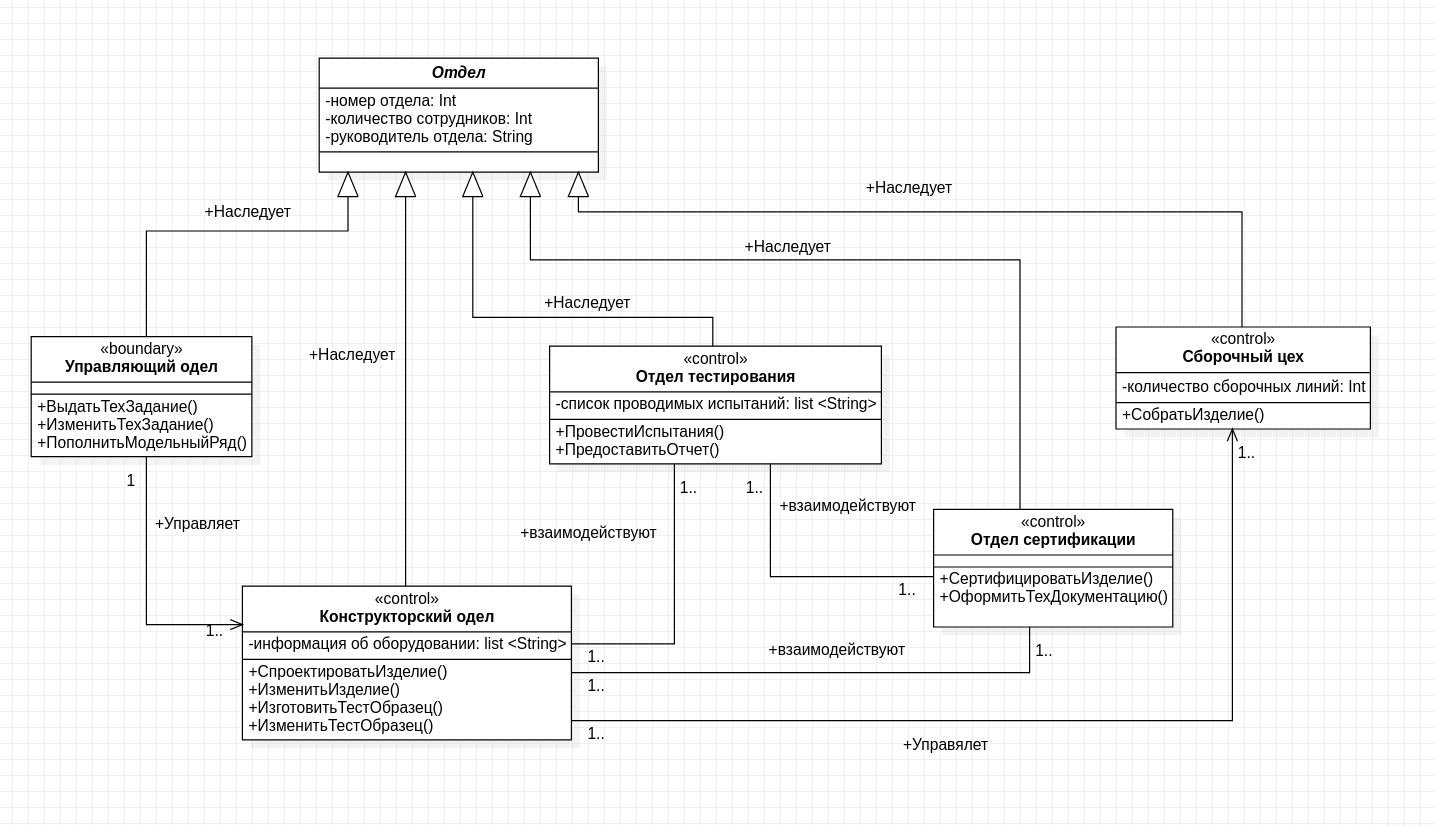
\includegraphics[width=0.9\linewidth]{images/classdiagram}
	\caption{Диаграмма Классов}
	\label{fig:classdiagram}
\end{figure}


\textit{Диаграмма классов является логическим представлением структуры модели, поэтому она должна содержать столько классов, сколько необходимо для реализации всего проекта. При этом для полного представления структуры модели необходимо установить и специфицировать отношения между классами.} 


\section{Особенности разработки диаграмм кооперации}
Диаграмма кооперации является разновидностью диаграммы взаимодействия, и в контексте языка UML описывает динамический аспект взаимодействия объектов при реализации отдельных вариантов использования. Активизировать рабочее окно диаграммы кооперации в программе \staruml можно несколькими способами:
\begin{itemize}
	\item выбрать соответствующий вариант, перейдя по следующим пунктам меню: \\$Model \to Add Diagram \to Communication Diagram$;
	\item нажать правую кнопку мыши на рабочей области и выбрать аналогичные пункты контекстного меню: $Add Diagram \to Communication Diagram$;
\end{itemize}

При этом появляется новое окно с чистым рабочим листом диаграммы кооперации и специальная панель инструментов, содержащая кнопки с изображением графических примитивов, необходимых для разработки диаграммы кооперации (рис. \ref{fig:toolboxcommunication}).  Назначение отдельных кнопок панели можно узнать из всплывающих подсказок.

% TODO: \usepackage{graphicx} required
\begin{figure}[h!]
	\centering
	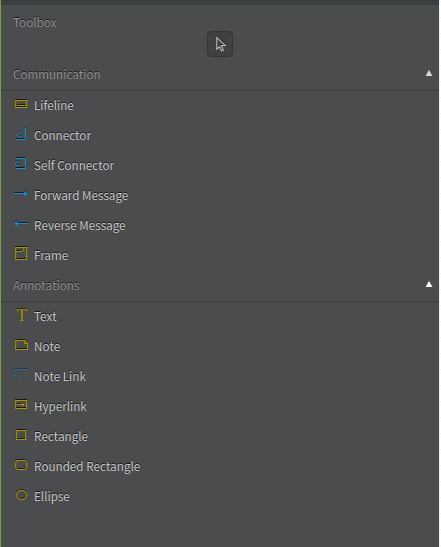
\includegraphics[width=0.5\linewidth]{images/toolboxcommunication}
	\caption{Communication Diagram: Панель инструментов}
	\label{fig:toolboxcommunication}
\end{figure}

В качестве примера рассматривается процесс построения диаграммы кооперации, которая представляет собой реализацию варианта использования <<Разработки новой модели велосипеда>> применительно к разрабатываемому проекту описания работы велосипедного предприятия. В модели данная диаграмма кооперации соответствует этому варианту использования и может быть размещена в представлении вариантов использования (Use Case View).

После активизации новой диаграммы кооперации одним из описанных выше способов следует в качестве имени данной диаграммы задать: <<Разработка новой модели велосипеда>>.

В общем случае работа с диаграммой кооперации состоит в добавлении объектов, связей и сообщений, а также редактировании их свойств.
\subsubsection*{Добавление объекта на диаграмму кооперации и редактирование его свойств}
Добавить объект на диаграмму кооперации можно стандартным образом с помощью соответствующей кнопки на специальной панели инструментов. Однако, в случае наличия построенной ранее диаграммы классов, более удобным представляется следующий способ. 

В обозревателе проекта выделить необходимый класс и, удерживая нажатой левую кнопку мыши, перетащить изображение пиктограммы класса из браузера на свободное место рабочего листа диаграммы кооперации. В результате этих действий на диаграмме кооперации появится изображение объекта с именем класса и маркерами изменения его геометрических размеров (рис. \ref{fig:communicationfield}).

% TODO: \usepackage{graphicx} required
\begin{figure}[h!]
	\centering
	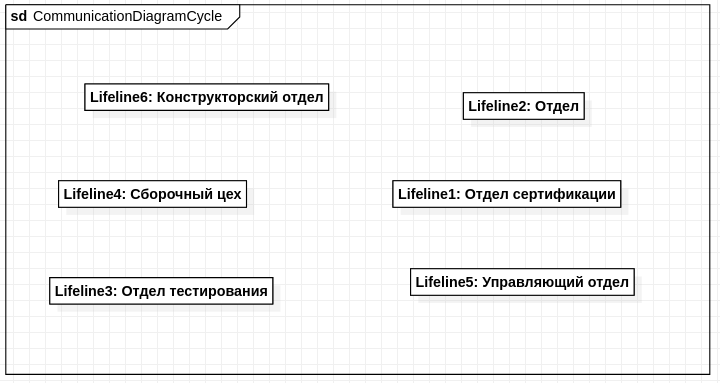
\includegraphics[width=0.8\linewidth]{images/communicationfield}
	\caption{Объекты диаграммы кооперации}
	\label{fig:communicationfield}
\end{figure}


По умолчанию каждый добавляемый объект считается анонимным. При необходимости можно задать собственное имя объекта, для чего двойным щелчком на изображении объекта на диаграмме кооперации следует вызвать контекстное меню свойств этого объекта (рис. \ref{fig:communicationobject}).

% TODO: \usepackage{graphicx} required
\begin{figure}[h!]
	\centering
	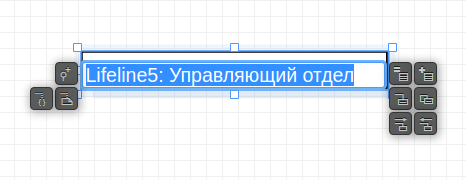
\includegraphics[width=0.7\linewidth]{images/communicationobject}
	\caption{Контекстное меню}
	\label{fig:communicationobject}
\end{figure}


Для объекта выбранного класса можно задавать: собственное имя объекта, особенности его реализации и множественность экземпляров.
\label{multinstance}
При необходимости можно представить объект в форме мультиобъекта. Для этого следует поставить галочку у свойства \textit{isMultinstance } (Несколько экземпляров). Однако для объекта класса \textit{Управляющий отдел} и это свойство следует оставить пустым, поскольку данный объект присутствует в модели в единственном экземпляре.

\subsubsection*{Добавление сообщения и редактирование его свойств}
Для добавления сообщения между предварительно размещенными на диаграмме объектами нужно с помощью левой кнопки мыши нажать кнопку с изображением связи на специальной панели инструментов, отпустить левую кнопку мыши, щелкнуть левой кнопкой мыши на изображении одного объекта на диаграмме и отпустить ее на изображении другого объекта.

В результате этих действий на диаграмме появится изображение связи, например, соединяющей объект класса \textit{Управляющий Отдел} с объектом класса \textit{Конструкторский отдел} (рис. \ref{fig:message1}). После этого следует выполнить операцию \textit{Select Operation} контекстного меню сообщения, в результате чего появляется вложенный список с предложением выбрать одну из операций целевого класса для спецификации имени сообщения (рис. \ref{fig:message2}).

% TODO: \usepackage{graphicx} required
\begin{figure}[h!]
	\centering
	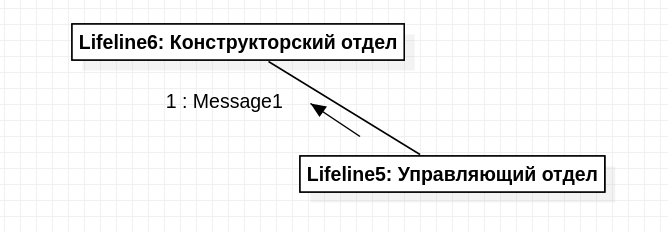
\includegraphics[width=0.7\linewidth]{images/message1}
	\caption{Изображение связи}
	\label{fig:message1}
\end{figure}

% TODO: \usepackage{graphicx} required
\begin{figure}[h!]
	\centering
	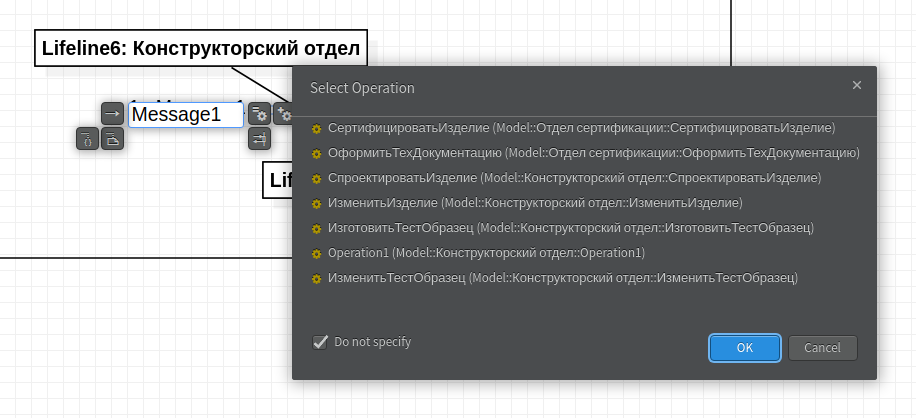
\includegraphics[width=0.7\linewidth]{images/message2}
	\caption{Выбор сообщения (метода)}
	\label{fig:message2}
\end{figure}

Для рассматриваемой модели предприятия для первого сообщения следует выбрать операцию \textit{ОформитьТехДокументацию()}. После выбора операции для данного сообщения оно добавляется в список сообщений данной связи, а рядом с линией связи на диаграмме кооперации появится стрелка с номером и именем этого сообщения (рис. \ref{fig:message3}).

% TODO: \usepackage{graphicx} required
\begin{figure}[h!]
	\centering
	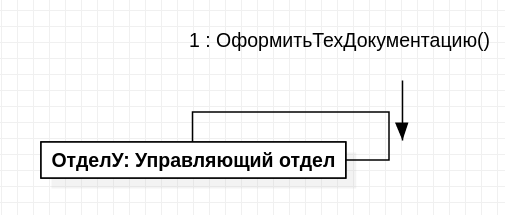
\includegraphics[width=0.7\linewidth]{images/message3}
	\caption{Рефлексивное сообщение}
	\label{fig:message3}
\end{figure}

Характеристика отдельных свойств синхронизации сообщений и графическое изображение соответствующих стрелок сообщений приводится в следующей таблице (табл. \ref{tab:messages}).

\begin{table}[h!]

	\begin{tabular}{|m{0.3\linewidth}|m{0.6\linewidth}|}
		\hline
	\textbf{Название свойства} & \textbf{Назначение свойства} \\ \hline
		Simple 
		(Простое) & Данное сообщение выполняется в одном потоке управления. Это свойство задается добавляемому на диаграмму сообщению по умолчанию \\ \hline
		Synchronous 
		(Синхронное) & После передачи данного сообщения клиент ожидает ответа от объекта-приемника о результате выполнения соответствующей операции \\ \hline
		Balking 
		(С отказом) & После передачи данного сообщения объект-приемник отказывает клиенту в выполнении соответствующей операции, если он занят выполнением других операций \\ \hline
		Timeout 
		(С ожиданием) & После передачи данного сообщения объект-приемник может поместить данное сообщение в очередь с ограниченным временем ожидания, если он занят выполнением других операций \\ \hline
		Procedure Call
		(Вызов процедуры) & Клиент посылает данное сообщение объекту-приемнику и, чтобы продолжить свою работу ожидает, пока вся дальнейшая вложенная последовательность сообщений не будет обработана приемником \\ \hline
		Asynchronous
		(Асинхронное) & Клиент посылает данное сообщение и продолжает свою работу, не ожидая подтверждения от объекта-приемника о получении этого сообщения. При этом соответствующая операция может быть как выполнена, так и не выполнена \\ \hline
		Return (Возврат) & Данное сообщение посылается клиенту после окончания выполнения вызова процедуры \\ \hline
	\end{tabular}
	\caption{Свойства сообщений}
	\label{tab:messages}
\end{table}
\newpage
\subsubsection*{Окончательное построение диаграммы последовательности модели предприятия по производству велосипедов}
Для завершения построения диаграммы последовательности рассматриваемого примера следует описанным выше способом добавить оставшиеся объекты и сообщения. С этой целью следует выполнить следующие действия:
\begin{enumerate}
	\item Добавить объекты класссов \textit{Отдел сертификации, Сборочный цех, , Отдел тестирования};
	\item Указать объекты всех классов как мультиобъекты, выбрав соответствующий параметр в секции \textit{Editors};
	\item Добавить следующие сообщения между классами:
	\begin{itemize}
		\item ОформитьТехЗадание() 
		\item СпроектироватьИзделие()
		\item ИзготовитьТестОбразец()
		\item ПровестиИспытания()
		\item ПредоставитьОтчет()
		\item СертифицироватьИзделие()
		\item ОформитьТехДокументацию()
		\item СобратьИзделие()
		\item ПополнитьМодельныйРяд()
	\end{itemize}
	\item Указать стереотипы для классов. В случае данного варианта использования класс \textit{Управляющий отдел} будет иметь стереотип \textit{<<border>>}, так как он является точкой инициализации и точкой окончания процесса. Все остальные классы составляют внутреннюю систему и имеют стереотип \textit{<<control>>}.
\end{enumerate}

При необходимости можно изменить порядок следования сообщений и их спецификацию, а также установить дополнительную синхронизацию сообщений и связать с сообщениями примечания, следует обратиться к Обозревателю Модели (\textit{Model Explorer}), в котором можно изменить порядок следования сообщений, выбрав пункт \textit{(Move Up/Move Down)} или воспользоваться сочетанием клавиш \texttt{Ctrl+Shift+Стрелка вверх}/\texttt{Ctrl+Shift+Стрелка вниз}.

Диаграмма кооперации, описывающая реализацию типичного хода событий варианта использования \textit{Разработка новой модели велосипеда} показана на рис. \ref{fig:communication}.

% TODO: \usepackage{graphicx} required
\begin{figure}[h!]
	\centering
	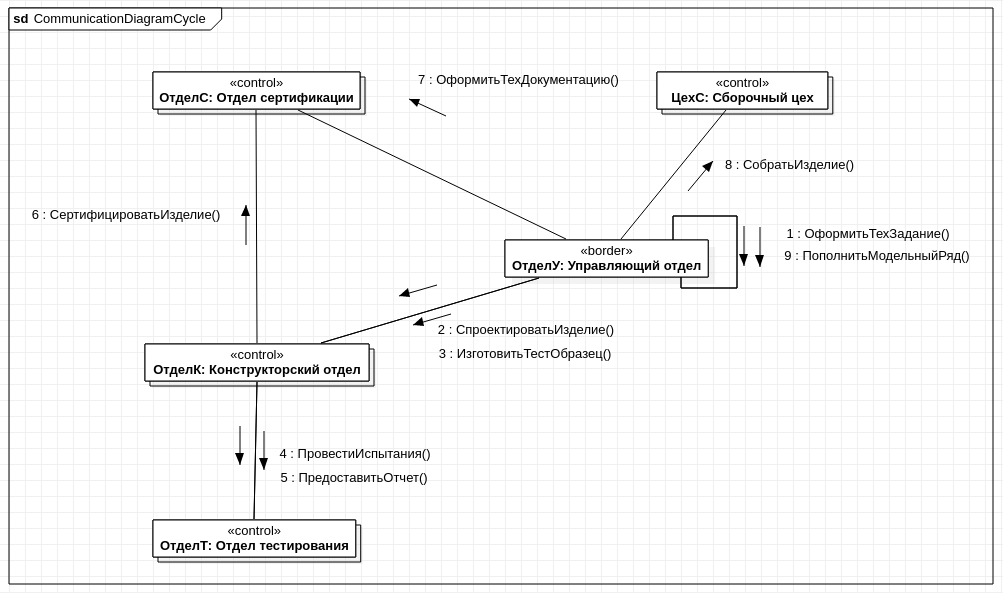
\includegraphics[width=1\linewidth]{images/communication}
	\caption{Диаграмма кооперации}
	\label{fig:communication}
\end{figure}

\section{Особенности разработки\\диаграммы последовательности}
Диаграмма последовательности является другой формой визуализации взаимодействия в модели и, как и диаграмма кооперации, оперирует объектами и сообщениями.

Основными элементами диаграммы последовательности являются обозначения объектов (прямоугольники с названиями объектов), вертикальные
<<линии жизни>> (англ. \textit{lifeline}), отображающие течение времени, прямоугольники, отражающие деятельность объекта или исполнение им определенной функции (прямоугольники на пунктирной <<линии жизни>>), и стрелки, показывающие обмен сигналами или сообщениями между объектами.

Активизировать рабочее окно диаграммы последовательности в среде разработки \staruml можно несколькими способами:
\begin{itemize}
	\item выбрать соответствующий вариант, перейдя по следующим пунктам меню: \\$Model \to Add Diagram \to Sequence Diagram$;
	\item нажать правую кнопку мыши на рабочей области и выбрать аналогичные пункты контекстного меню: $Add Diagram \to Sequence Diagram$;
\end{itemize}

При этом появляется новое окно с чистым рабочим листом диаграммы классов и специальная панель инструментов, содержащая кнопки с изображением графических примитивов, необходимых для разработки диаграммы последовательности (табл. \ref{tab:toolboxsequence}). Назначение отдельных кнопок панели можно узнать из всплывающих подсказок.

\begin{table}[h!]
	
	\begin{tabular}{|l|m{0.6\linewidth}|}
		\hline
		\textbf{Всплывающая подсказка}&\textbf{Назначение кнопки} \\ \hline
		Selection Tool&Превращает изображение курсора в форму стрелки для последующего выделения элементов на диаграмме \\ \hline
		Text Box& Добавляет на диаграмму текстовую область \\ \hline
		Note& Добавляет на диаграмму примечание \\ \hline
		Anchor Note to Item & Добавляет на диаграмму связь примечания с соответствующим графическим элементом диаграммы \\ \hline
		Object &Добавляет на диаграмму объект \\ \hline
		Object Message& Добавляет на диаграмму простое сообщение \\ \hline
		Message To Self&Добавляет на диаграмму рефлексивное сообщение \\ \hline
		Return Message&Добавляет на диаграмму сообщение типа возврата из вызова процедуры \\ \hline
		Destruction Marker&Добавляет на диаграмму символ уничтожения объекта \\ \hline
		Procedure Call&Добавляет на диаграмму сообщение типа вызова процедуры \\ \hline
		Asynchronous Message&Добавляет на диаграмму асинхронное сообщение  \\ \hline
	\end{tabular}
	\caption{Диаграмма последовательности: Панель инструментов}
	\label{tab:toolboxsequence}
\end{table}

\subsubsection*{Добавление объекта на диаграмму последовательности и редактирование его свойств}
Добавить объект на диаграмму последовательности можно как стандартным образом с помощью соответствующей кнопки на специальной панели инструментов, так и более удобным способом --- с помощью перетаскивания изображения пиктограммы класса из браузера на свободное место рабочего листа диаграммы последовательности.

В результате этих действий на диаграмме последовательности появится изображение объекта с именем класса, маркерами изменения его геометрических размеров и вертикальной пунктирной линией, означающей линию жизни этого объекта (рис. \ref{fig:sequenceobjects}).

\vspace{5ex}
% TODO: \usepackage{graphicx} required
\begin{figure}[h!]
	\centering
	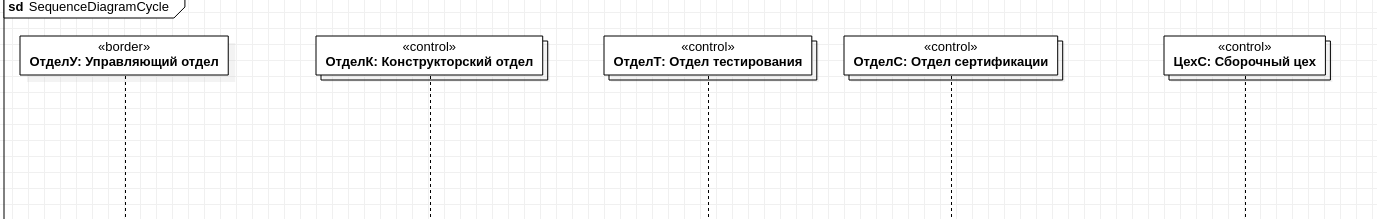
\includegraphics[width=1\linewidth]{images/sequenceobjects}
	\caption{Объекты диаграммы последовательности}
	\label{fig:sequenceobjects}
\end{figure}

Так же как и для диаграммы кооперации, для диаграммы последовательности каждый добавляемый объект по умолчанию считается анонимным. При необходимости можно задать собственное имя объекта, для чего уже известным способом (например, двойным щелчком на изображении объекта на диаграмме) следует вызвать диалоговое окно свойств объекта или обратиться к секции \textit{Editors}.


При необходимости можно представить объект в форме мультиобъекта. Для этого следует выбрать отметку у свойства isMultinstance (Несколько экземпляров), аналогично тому, как это было достигнуто при проектировании \hyperref[multinstance]{диаграммы кооперации}.

\subsubsection*{Добавление связи и редактирование ее свойств}
Для добавления рефлексивной связи (отправки рефлексивного сообщения) следует выбрать соответствующий инструмент  (\textit{Self Message}) на панели и нажать левой кнопкой мыши на объект класса в рабочей области диаграммы последовательности. Далее следует внести название связи в предлагаемое поле. В конкретном примере показан процесс создания рефлексивной связи класса \textit{Управляющий отдел} (рис. \ref{fig:sequenceaction2}).

% TODO: \usepackage{graphicx} required
\begin{figure}[h!]
	\centering
	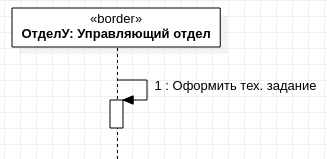
\includegraphics[width=0.7\linewidth]{images/sequenceaction2}
	\caption{Рефлексивная связь}
	\label{fig:sequenceaction2}
\end{figure}

Для добавления связи между предварительно размещенными на диаграмме объектами нужно с помощью левой кнопки мыши нажать кнопку с изображением связи на специальной панели инструментов, отпустить левую кнопку мыши, щелкнуть левой кнопкой мыши на изображении одного объекта на диаграмме и отпустить ее на изображении другого объекта. 

В результате этих действий на диаграмме появится изображение связи, например, соединяющей объект класса \textit{Управляющий отдел} с объектом класса \textit{Конструкторский отдел} (рис. \ref{fig:sequenceaction1}). При этом изображение линии жизни у соответствующей пары объектов изменится на изображение фокуса управления.

% TODO: \usepackage{graphicx} required
\begin{figure}[h!]
	\centering
	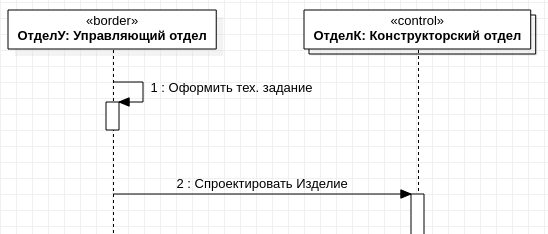
\includegraphics[width=0.7\linewidth]{images/sequenceaction1}
	\caption{Отображение связи между объектами}
	\label{fig:sequenceaction1}
\end{figure}

После добавления имени связи можно перейти к дополнительным параметрам. Например, задать имя ассоциации, видимость соответствующей пары объектов и наличие общих ролей. Для редактирования свойств связи следует обратиться к вспомогательной секции \textit{Editors}, расположенной справа от рабочей области (рис. \ref{fig:sequenceeditors}).

% TODO: \usepackage{graphicx} required
\begin{figure}[h!]
	\centering
	\includegraphics[width=0.5\linewidth]{images/sequenceeditors}
	\caption{Свойства связи}
	\label{fig:sequenceeditors}
\end{figure}

Построение диаграммы последовательности сводится к добавлению и редактированию свойств отдельных объектов и сообщений. Доступ к окну спецификации свойств соответствующих элементов возможен также либо через контекстное меню, либо с помощью секции меню \textit{Editors}. При добавлении сообщений на диаграмму последовательности они получают по умолчанию свой номер в общей последовательности сообщений.

Для изменении порядка следования сообщений следует обратиться к Обозревателю Модели (\textit{Model Explorer}), выбрав пункт \textit{(Move Up/Move Down)} или воспользоваться сочетанием клавиш \texttt{Ctrl+Shift+Стрелка вверх}/\texttt{Ctrl+Shift+Стрелка вниз}. При этом список сообщений автоматически перестроен. См. рис. \ref{fig:sequenceexplorer}.

% TODO: \usepackage{graphicx} required
\begin{figure}[h!]
	\centering
	\includegraphics[width=0.5\linewidth]{images/sequenceexplorer}
	\caption{Меню обозревателя модели}
	\label{fig:sequenceexplorer}
\end{figure}

\subsubsection*{Управление сложными взаимодействиями с фрагментами последовательности}

Диаграмма последовательности в нотации UML предусматривает добавление сложных фрагментов для реализации таких сценариев использования как циклическое действие, альтернативное действие, справочный сегмент. \staruml также располагает средствами для использования данных фрагментов. 

Рассмотрим правила использования данных фрагментов на примере системы <<Банкомат>>.

Фрагмент последовательности представлен в виде рамки, обрамляющей участок взаимодействия между объектами (как показано в примерах ниже) на диаграмме последовательности.

Он используется для более структурированного отображения сложных взаимодействий, таких как альтернативные потоки и циклы. В верхнем левом углу фрагмента расположен оператор. Этот оператор (оператор фрагмента) указывает на вид фрагмента.
\paragraph{Альтернативы}

Фрагмент альтернативной комбинации используется, когда необходимо сделать выбор между двумя или более последовательностями сообщений. Он моделирует логику <<если, то еще>>.

Альтернативный фрагмент представляет собой большой прямоугольник или кадр, который задается упоминанием 'alt' в окошке с названием кадра (так называемый оператор фрагмента).

Чтобы показать две или более альтернативы, больший прямоугольник затем делится на то, что называется операндов взаимодействия, используя пунктирную линию, как показано на примере диаграммы последовательности выше. Каждый операнд имеет защитное ограждение, которое проверяется и размещается в верхнем левом углу операндов.

% TODO: \usepackage{graphicx} required
\begin{figure}[h!]
	\centering
	\includegraphics[width=0.6\linewidth]{images/framealt}
	\caption{Пример альтернативного фрагмента}
	\label{fig:framealt}
\end{figure}


\paragraph{Варианты}

Фрагмент комбинации опций используется для указания последовательности, которая будет происходить только при определенном условии, в противном случае последовательность не будет происходить. Оно моделирует утверждение “если тогда”.

Как и альтернативный фрагмент, фрагмент опции также представлен прямоугольной рамкой, в которой в окошке с названием помещается 'opt'.

В отличие от альтернативного фрагмента, фрагмент опции не делится на два или более операндов. Вариант защиты расположен в верхнем левом углу.

\paragraph{Loops}

Loop фрагмент используется для представления повторяющейся последовательности.

В квадратных скобках секции Loop можно разместить условия выхода из цикла или защитные условия \textit{(Guard Condition)}. 

Если это защита от минимальных итераций, то шлейф должен выполняться не меньше указанного числа, а если это защита от максимальных итераций, то шлейф не должен выполняться больше указанного числа.

(Пример фрагмента цикла приведен ниже в шаблонах последовательных диаграмм и разделе с примерами)

\paragraph{Справочный фрагмент}

Вы можете использовать фрагмент ссылки для управления размером больших последовательных диаграмм. Это позволяет повторно использовать часть одной диаграммы последовательностей в другой, или, другими словами, можно ссылаться на часть диаграммы в другой диаграмме, используя фрагмент ref-фрагмента.

Для указания ссылочного фрагмента необходимо в окошке с названием кадра указать 'ref', а внутри кадра --- название диаграммы последовательности, на которую делается ссылка.

% TODO: \usepackage{graphicx} required
\begin{figure}[h!]
	\centering
	\includegraphics[width=0.6\linewidth]{images/frameoptref}
	\caption{Пример справочного и вариантного фрагмента}
	\label{fig:frameoptref}
\end{figure}

\subsubsection*{Добавление фрагментов последовательности}

При разработке рассматриваемой диаграммы последовательности, описывающей вариант использования <<Разработка новой модели велосипеда>> мы также использовали фрагменты для отражения альтернативного выбора и циклически выполняемых действий.

Для добавления такого фрагмента следует выбрать инструмент \textit{Combined Fragment} на панели и разместить его на рабочей области. 
Изменить тип фрагмента можно в секции \textit{Editors}, выбрав один из вариантов, предлагаемых в выпадающем списке. См. рис. \ref{fig:sequenceeditors2}.

% TODO: \usepackage{graphicx} required
\begin{figure}[h!]
	\centering
	\includegraphics[width=0.5\linewidth]{images/sequenceeditors2}
	\caption{Настройки фрагмента}
	\label{fig:sequenceeditors2}
\end{figure}

\subsubsection*{Окончательное построение диаграммы последовательности модели предприятия}
Для завершения построения диаграммы последовательности рассматриваемого примера следует описанным выше способом добавить оставшиеся объекты и сообщения, которые упоминались в диаграмме кооперации.

Фрагмент диаграммы последовательности, описывающая реализацию типичного хода событий варианта использования <<Разработка новой модели велосипеда>> для модели предприятия, показан на рис. \ref{fig:sequence}.

% TODO: \usepackage{graphicx} required
\begin{figure}[h!]
	\centering
	\includegraphics[width=1\linewidth]{images/sequence}
	\caption{Диаграмма последовательности}
	\label{fig:sequence}
\end{figure}
\newpage
\section{Особенности разработки диаграммы состояний}
Диаграмма состояний --- это, по существу, диаграмма состояний из теории автоматов со стандартизированными условными обозначениями, которая может определять множество систем от компьютерных программ до бизнес-процессов. Используются следующие условные обозначения:
\begin{itemize}
	\item Круг, обозначающий начальное состояние;
	\item Окружность с маленьким кругом внутри, обозначающая конечное состояние (если есть);
	\item Скруглённый прямоугольник, обозначающий состояние. Верхушка прямоугольника содержит название состояния. В середине может быть горизонтальная линия, под которой записываются активности, происходящие в данном состоянии;
	\item Стрелка, обозначающая переход. Название события (если есть), вызывающего переход, отмечается рядом со стрелкой. Охраняющее выражение может быть добавлено перед <</>> и заключено в квадратные скобки, что значит, что это выражение должно быть истинным, чтобы переход имел место. Если при переходе производится какое-то действие, то оно добавляется после <</>> (название\_события[охраняющее\_выражение]/действие);
	\item Толстая горизонтальная линия с либо множеством входящих линий и одной выходящей, либо одной входящей линией и множеством выходящих. Это обозначает объединение и разветвление соответственно.
\end{itemize}


Начать построение диаграммы состояний для выбранного элемента модели или моделируемой системы в целом можно одним из следующих способов:
\begin{itemize}
	\item выбрать соответствующий вариант, перейдя по следующим пунктам меню: \\$Model \to Add Diagram \to Statechart Diagram$;
	\item нажать правую кнопку мыши на рабочей области и выбрать аналогичные пункты контекстного меню: $Add Diagram \to Statechart Diagram$;
\end{itemize}

Продолжая разработку проекта по моделированию предприятия по производству велосипедов, можно приступить к разработке новой диаграммы состояний. С этой целью для диаграммы состояний модели предприятия зададим имя StatechartDiagramCycle.

В результате выполнения этих действий появляется новое окно с чистым рабочим листом диаграммы состояний и специальная панель инструментов, содержащая кнопки с изображением графических элементов модели, необходимых для разработки диаграммы состояний. Приведем назначение основных инструментов в таблице \ref{tab:toolboxstatechart}. Назначение отдельных кнопок панели можно узнать из всплывающих подсказок.

\begin{table}[h!]

	\begin{tabular}{|l|m{0.6\linewidth}|}
		\hline
		\textbf{Всплывающая подсказка} & \textbf{Назначение кнопки} \\ \hline
		Text Box & Добавляет на диаграмму текстовую область \\ \hline
		Note & Добавляет на диаграмму примечание \\ \hline
		Simple State & Добавляет на диаграмму состояние \\ \hline
		Initial State & Добавляет на диаграмму начальное состояние \\ \hline
		Final State & Добавляет на диаграмму конечное состояние \\ \hline
		Transition & Добавляет на диаграмму переход \\ \hline
		Self Transition & Добавляет на диаграмму рефлексивный переход \\ \hline
		Join/Fork & Добавляет на диаграмму символ для описания параллельного перехода \\ \hline
		Choice & Добавляет на диаграмму символ принятия решения для альтернативных переходов \\ \hline
	\end{tabular}
	\caption{Диаграмма состояний: Назначения инструментов}
	\label{tab:toolboxstatechart}
\end{table}

Полный список используемых инструментов можно увидеть на рисунке \ref{fig:statecharttoolbox}.
\newpage
% TODO: \usepackage{graphicx} required
\begin{figure}[h!]
	\centering
	\includegraphics[width=0.4\linewidth]{images/statecharttoolbox}
	\caption{Диаграмма состояний: Панель инструментов}
	\label{fig:statecharttoolbox}
\end{figure}
%\newpage
\subsubsection*{Добавление состояния на диаграмму состояний и редактирование его свойств}
Для добавления состояния на диаграмму состояний необходимо с помощью левой кнопки мыши нажать кнопку с изображением пиктограммы состояния на специальной панели инструментов, отпустить левую кнопку мыши и щелкнуть левой кнопкой мыши на свободном месте рабочего листа диаграммы. На диаграмме появится изображение состояния с маркерами изменения его геометрических размеров и предложенным средой именем по умолчанию, которое разработчику следует изменить.

 Для диаграммы состояний модели предприятия в качестве имени первого добавленного состояния изменим предложенное программой по умолчанию имя \textit{State1} на \textit{Разработка Технического задания} (рис \ref{fig:statechartinit}). Задать имя элемента можно либо непосредственно при добавлении нового состояния на диаграмму состояний, либо открыв окно спецификации свойств нового состояния.

% TODO: \usepackage{graphicx} required
\begin{figure}[h!]
	\centering
	\includegraphics[width=0.7\linewidth]{images/statechartinit}
	\caption{Добавление состояния на диаграмму}
	\label{fig:statechartinit}
\end{figure}


\subsubsection*{Добавление перехода и редактирование его свойств}
Для добавления перехода между двумя состояниями нужно с помощью левой кнопки мыши нажать кнопку с изображением перехода на специальной панели инструментов, отпустить левую кнопку мыши, щелкнуть левой кнопкой мыши на изображении исходного состояния на диаграмме и отпустить ее на изображении целевого состояния. 

В результате этих действий на диаграмме появится изображение перехода, соединяющего два выбранных состояния. Продолжая разработку модели предприятия, добавим на диаграмму состояний начальное состояние \textit{(Initial State)} и соединим его переходом с состоянием \textit{Разработка Технического задания} (рис. \ref{fig:statechartfirst}). Для добавления переходу имени следует дважды кликнуть левой кнопкой мыши на изображении стрелки и ввести условия, названия, охранные выражения присущие данному переходу.

% TODO: \usepackage{graphicx} required
\begin{figure}[h!]
	\centering
	\includegraphics[width=0.5\linewidth]{images/statechartfirst}
	\caption{Добавление перехода на диаграмму}
	\label{fig:statechartfirst}
\end{figure}

Состояние может содержать только имя или имя и дополнительно список внутренних действий. Список внутренних действий содержит перечень действий или деятельностей, которые выполняются во время нахождения объекта в данном состоянии. Данный список фиксированный. Список основных действий включает следующие значения:
\begin{itemize}
	\item entry ---действие, которое выполняется в момент входа в данное состояние (входное действие);
	\item exit --- действие, которое выполняется в момент выхода из данного состояния (выходное действие);
	\item do --- выполняющаяся деятельность (<<do activity>>) в течение всего времени, пока объект находится в данном состоянии
	\item defer --- событие, обработка которого предписывается в другом состоянии, но после того, как все операции в текущем будут завершены.
\end{itemize}
\subsubsection*{Узлы ветвления и объединения}
Узлы ветвления и объединения аналогичны узлам на диаграмме деятельности. На диаграмме состояний обычно данные подсостяония используются для распараллеливания переходов в композитных состояниях, о которых речь пойдет позже. После срабатывания перехода моделируемый объект одновременно будет находиться во всех целевых состояниях этого перехода. 

Варианты принятия решений на диаграмме состояний могут быть показаны также как и на диаграмме деятельности с помощью узла выбора. При этом переход в состояние выбора должен быть триггерным и содержать имя события. Переходы из псевдосостояния выбора в целевые состояния должны содержать сторожевые условия. Переход, который должен срабатывать, если ни одно из условий не примет значение <<истина>> должен содержать метку <<else>>. 

В дальнейшем мы используем узел ветвления при построении диаграммы состояний для модели рассматриваемого предприятия по производству велосипедов.

\subsubsection*{Сложные и простые состояния}

На диаграмме могут быть представлены как простые состояния, так и сложные состояния. Сложные или составные состояния \textit{(composite state)}  включают в себя вложенные подсостояния.  Декомпозиция сложного состояния может осуществляться как на основной диаграмме, так и отдельно. Приведем пример сложного состояния, описанного при построении модели рассматриваемого предприятия (рис. \ref{fig:statechartcomposestate}).

% TODO: \usepackage{graphicx} required
\begin{figure}
	\centering
	\includegraphics[width=0.4\linewidth]{images/statechartcomposestate}
	\caption{Составное состояние}
	\label{fig:statechartcomposestate}
\end{figure}


\subsubsection*{Последовательные и параллельные состояния}

\textbf{Последовательные подсостояния/состояния} \textit{(sequential substates)} используются для моделирования такого поведения объекта, во время которого в каждый момент времени объект может находиться в одном и только одном подсостояний. Поведение объекта в этом случае представляет собой последовательную смену подсостояний, начиная от начального и заканчивая конечным подсостояниями.

\textbf{Параллельные подсостояния/состояния} \textit{(concurrent substates)} позволяют специфицировать два и более подавтомата, которые могут выполняться параллельно внутри составного события. Каждый из подавтоматов занимает некоторую область (регион) внутри составного состояния.

Переходы могут осуществляться как в само композитное состояние, так и в одно из его подсостояний. Таким образом, переход, стрелка которого соединена с границей некоторого составного состояния, обозначает переход в составное состояние. Он эквивалентен переходу в начальное состояние каждого из подавтоматов.

Переход, выходящий из составного состояния относится к каждому из вложенных подсостояний. Это означает, что объект может покинуть составное суперсостояние, находясь в любом из его подсостояний. Если необходимо указать конкретное подсостояние из которого может осуществиться выход из композитного состояния, достаточно добавить переход от подсостояния в целевое состояние.

Для данной системы состояния <<\textit{Изготовление вилки}>> и <<\textit{Изготовление рамы}>> могут быть рассмотрены как те, в которых система может находиться одновременно. С этой целью, используя инструменты \textit{Fork} и \textit{Join} построим узел параллельного перехода. См. рис. \ref{fig:statechartparallel}.
% TODO: \usepackage{graphicx} required
\begin{figure}[h!]
	\centering
	\includegraphics[width=0.5\linewidth]{images/statechartparallel}
	\caption{параллельные состояния}
	\label{fig:statechartparallel}
\end{figure}

\subsubsection*{Окончательное построение диаграммы состояний модели предприятия}
Для завершения построения диаграммы состояний рассматриваемого примера следует, основываясь на построенных диаграммах последовательности и кооперации, описанным выше способом добавить оставшиеся состояния и описать переходы между ними.

Диаграмма состояний для рассматриваемой модели предприятия будет иметь следующий вид (рис. \ref{fig:statechart}).
% TODO: \usepackage{graphicx} required
\begin{figure}[h!]
	\centering
	\includegraphics[width=1\linewidth]{images/statechart}
	\caption{Диаграмма состояний}
	\label{fig:statechart}
\end{figure}

\section{Особенности разработки диаграммы деятельности}
Диаграмма деятельности в среде \staruml, так же как и диаграмма состояний, может относиться к отдельному классу, операции класса, варианту использования, пакету или представлению. Начать построение диаграммы деятельности для выбранного элемента модели или моделируемой системы в целом можно одним из следующих способов:
\begin{itemize}
	\item выбрать соответствующий вариант, перейдя по следующим пунктам меню: \\$Model \to Add Diagram \to Activity Diagram$;
	\item нажать правую кнопку мыши на рабочей области и выбрать аналогичные пункты контекстного меню: $Add Diagram \to Activity Diagram$;
\end{itemize}

В результате выполнения этих действий появляется новое окно с чистым рабочим листом диаграммы деятельности и специальная панель инструментов, содержащая кнопки с изображением графических элементов, необходимых для разработки диаграммы деятельности (табл. \ref{tab:activitytoolbox}). Назначение отдельных кнопок панели можно узнать из всплывающих подсказок.

\begin{table}[htbp]

	\begin{tabular}{|l|m{0.6\linewidth}|}
		\hline
		\textbf{Всплывающая подсказка} &\textbf{ Назначение кнопки} \\ \hline
		Selection Tool & Превращает изображение курсора в форму стрелки для последующего выделения элементов на диаграмме \\ \hline
		Text Box & Добавляет на диаграмму текстовую область \\ \hline
		Note & Добавляет на диаграмму примечание \\ \hline
		Note Link & Добавляет на диаграмму связь примечания с соответствующим графическим элементом диаграммы \\ \hline
		Action & Добавляет на диаграмму состояние \\ \hline
		Initial & Добавляет на диаграмму начальное состояние \\ \hline
		Final & Добавляет на диаграмму конечное состояние \\ \hline
		Join/Fork & Добавляет на диаграмму символ для описания параллельного процесса \\ \hline
		Merge/Decison & Добавляет на диаграмму символ принятия решения для альтернативных переходов \\ \hline
	\end{tabular}
	\caption{Диаграмма активности: Назначение основных инструментов}
	\label{tab:activitytoolbox}
\end{table}

Более полный список предоставляемых инструментов можно видеть на рисунке \ref{fig:activitytoolbox}.
% TODO: \usepackage{graphicx} required
\begin{figure}[h!]
	\centering
	\includegraphics[width=0.5\linewidth]{images/activitytoolbox}
	\caption{Диаграмма Активности: Панель инструментов}
	\label{fig:activitytoolbox}
\end{figure}

Следует отметить, что в проектах реинжиниринга и документирования бизнес-процессов диаграмма деятельности является основным средством визуализации бизнес-процессов в контексте языка UML. 

Так как изучаемый процесс по производству новой модели велосипеда на производстве может быть представлен как бизнес-процесс, то мы можем рассмотреть особенности разработки диаграмм деятельности в среде \staruml на данном примере. 

Повторимся, что наиболее подходящим типом диаграмм для визуального представления схем выполнения бизнес-процессов являются диаграммы деятельности, на которых дополнительно размещаются так называемые дорожки \textit{(\textbf{Swimlane})}. Назначение \textbf{дорожек} состоит в том, чтобы указать зоны ответственности за выполнения отдельных деятельностей в рамках моделируемого бизнес-процесса. 
В качестве имен дорожек используются либо названия подразделений (департаментов) рассматриваемой компании, либо названия отдельных должностей сотрудников тех или иных подразделений.

Проекты по моделированию бизнес-процессов могут выполняться либо с целью реорганизации или реинжиниринга компании, либо с целью документирования бизнес-процессов. Особенности данных проектов заключаются в том, что в обоих случаях необходимо построить модели бизнес-процессов некоторой существующей компании. Чтобы акцентировать внимание на подобных проектах, их часто называют проектами типа \textit{<<As is>> (<<Как есть>>)}. Соответственно проекты по разработке новых продуктов или моделей новых систем называют проектами типа \textit{<<To be>>} \textit{(<<Как должно быть>>)}.

Выполнение проектов типа\textit{ <<Как есть>>} по моделированию бизнес-процессов в большинстве случаев начинают с построения диаграмм деятельности, которые служат для графического представления схем выполнения бизнес-процессов и документооборота рассматриваемой компании. После этого, исходя из требований проекта, разрабатывается модель диаграммы вариантов использования и выполняется реорганизация бизнес-процессов. Наконец, в случае необходимости разработки или внедрения корпоративной информационной системы, строятся диаграмма классов, диаграммы взаимодействия и компонентов, которые служат основой для программной реализации соответствующего проекта.

Таким образом, первый этап выполнения проектов типа \textit{<<Как есть>>} связан с построением моделей существующих бизнес-процессов компании в форме диаграмм деятельности. В качестве примера проекта этого типа рассматривается модель бизнес-процесса по разработке новой серийной модели велосипеда на предприятии. Хотя данный пример имеет упрощенный характер, он позволяет наглядно представить основные особенности моделирования бизнес-процессов в нотации языка UML с использованием средства \staruml.

\subsubsection*{Добавление деятельности на диаграмму деятельности и редактирование ее свойств}
Для добавления деятельности на диаграмму деятельности нужно с помощью левой кнопки мыши нажать кнопку с изображением пиктограммы деятельности \textit{(Action)} на специальной панели инструментов, отпустить левую кнопку мыши и щелкнуть левой кнопкой мыши на свободном месте рабочего листа диаграммы. 

На диаграмме появится изображение деятельности с маркерами изменения его геометрических размеров и предложенным средой именем по умолчанию, которое разработчику следует изменить. В результате этих действий на диаграмме появится изображение деятельности с именем \textit{Action1}, предложенное программой по умолчанию. Начиная построение диаграммы деятельности модели предприятия, для первой добавленной деятельности зададим имя \textit{Оформить тех. задание} (рис. \ref{fig:activityaction}).

% TODO: \usepackage{graphicx} required
\begin{figure}[h!]
	\centering
	\includegraphics[width=0.6\linewidth]{images/activityaction}
	\caption{Диаграмма активности. Добавление активности}
	\label{fig:activityaction}
\end{figure}


После добавления деятельности на диаграмму можно открыть меню \textit{Editiors}, где определить дополнительные свойства, доступные на соответствующих вкладках (рис. \ref{fig:activityeditors}).

% TODO: \usepackage{graphicx} required
\begin{figure}[h!]
	\centering
	\includegraphics[width=0.4\linewidth]{images/activityeditors}
	\caption{Диаграмма активности. Меню \textit{Editiors}}
	\label{fig:activityeditors}
\end{figure}

\subsubsection*{Добавление перехода и редактирование его свойств}

Добавление перехода на диаграмму деятельности полностью аналогично диаграмме состояний. А именно, для добавления перехода между двумя деятельностями нужно с помощью левой кнопки мыши нажать кнопку с изображением перехода (\textit{Control Flow}) на специальной панели инструментов, отпустить левую кнопку мыши, щелкнуть левой кнопкой мыши на изображении исходной деятельности на диаграмме и отпустить ее на изображении целевой деятельности (рис. \ref{fig:activityflow}).)

В результате этих действий на диаграмме появится изображение перехода, соединяющего две выбранных деятельности. Если в качестве одной из деятельностей является символ ветвления или соединения, то порядок добавления перехода сохраняется прежним.
% TODO: \usepackage{graphicx} required
\begin{figure}[h!]
	\centering
	\includegraphics[width=0.6\linewidth]{images/activityflow}
	\caption{Диаграмма активности. Добавление перехода}
	\label{fig:activityflow}
\end{figure}

После добавления перехода на диаграмму деятельности становятся доступными для редактирования его свойства в специальном диалоговом окне, которое можно открыть по двойному щелчку левой кнопкой мыши на изображении перехода.

При спецификации свойств переходов следует помнить, что все переходы на диаграмме деятельности является нетриггерными, т.е. не имеют имен событий. По этой причине поле ввода с именем \textit{Name} (Имя) для всех переходов должно оставаться пустым. Но все переходы, выходящие из символов ветвления (решения), должны иметь сторожевые условия.
\subsubsection*{Добавление дорожек на диаграмму деятельности}	
Для представления модели бизнес-процесса в форме диаграммы деятельности первоначально необходимо добавить на нее дорожки. Для добавления дорожки на диаграмму деятельности нужно с помощью левой кнопки мыши нажать кнопку с изображением пиктограммы дорожки(\textit{Swimlane}) на специальной панели инструментов, отпустить левую кнопку мыши и щелкнуть левой кнопкой мыши на свободном месте рабочего листа диаграммы. Причем программа \staruml располагает возможностью добавить как вертикальную дорожку, так и горизонтальную, что иногда может быть полезно при построении диаграммы активности.

В результате этих действий на диаграмме в области диаграммы появится изображение дорожки с вертикальной линией и именем дорожки \textit{ActivityPartition1} в верхней части, предложенное программой по умолчанию. Для задания имени дорожки следует дважды кликнуть левой кнопкой мыши на нее и вписать название в предложенную область (рис. \ref{fig:activityswimlane}).

% TODO: \usepackage{graphicx} required
\begin{figure}[h!]
	\centering
	\includegraphics[width=0.4\linewidth]{images/activityswimlane}
	\caption{Диаграмма активности. Добавление Swimlane}
	\label{fig:activityswimlane}
\end{figure}

Начиная практическую разработку модели бизнес-процесса разработки новой модели велосипеда, последовательно добавим на диаграмму деятельности дорожки с именами отдельных подразделений предприятия: \textit{Управляющий отдел, Конструкторский отдел, Отдел тестирования, Отдел сертификации, Сборочный цех.} (рис. \ref{fig:activityswimlaneall}).

% TODO: \usepackage{graphicx} required
\begin{figure}[h!]
	\centering
	\includegraphics[width=0.7\linewidth]{images/activityswimlaneall}
	\caption{Диаграмма активности. Добавление дорожек отделов}
	\label{fig:activityswimlaneall}
\end{figure}

После добавления дорожек на диаграмму состояний можно перейти к добавлению деятельностей и переходов. Переместим добавленные ранее активности на соответствующие дорожки (рис. \ref{fig:activityactivityonlane}).

% TODO: \usepackage{graphicx} required
\begin{figure}[h!]
	\centering
	\includegraphics[width=0.7\linewidth]{images/activityactivityonlane}
	\caption{Диаграмма активности. Добавление активности на Swimlane}
	\label{fig:activityactivityonlane}
\end{figure}


Данное расположение активностей будет означать, что деятельность \textit{Оформить тех. задание} выполняется в \textit{Управляющем отделе}, а деятельность \textit{Спроектировать изделие} --- в \textit{Конструкторском отделе.}
\subsubsection*{Построение диаграммы деятельности с дорожками для модели бизнес-процесса}
Для построения диаграммы деятельности с дорожками для рассматриваемой модели бизнес-процесса \textit{(разработка новой модели велосипеда)} следует добавить оставшиеся деятельности и переходы, описывающие данный процесс. 

Добавим активности на дорожки \textit{Управляющего отдела, Конструкторского отдела, Отдела тестирования, Отдела сертификации и Сборочного цеха} (см рис \ref{fig:activitydiagramswimlane}.)
% TODO: \usepackage{graphicx} required
\begin{figure}[h!]
	\centering
	\includegraphics[width=0.8\linewidth]{images/activitydiagramswimlane}
	\caption{Диаграмма активности с дорожками для модели бизнес-процесса}
	\label{fig:activitydiagramswimlane}
\end{figure}

\subsubsection*{Построение диаграммы деятельности с дорожками и потоком объектов}

Для построения диаграммы деятельности с дорожками и потоком объектов для рассматриваемой модели бизнес-процесса следует добавить на диаграмму объекты и стрелки потоков объектов. 

Для графического представления объектов	 используются прямоугольник класса, с тем отличием, что имя объекта подчеркивается. Далее после имени может указываться характеристика состояния объекта в прямых скобках. Такие прямоугольники объектов присоединяются к состояниям действия отношением зависимости пунктирной линией со стрелкой. Соответствующая зависимость определяет состояние конкретного объекта после выполнения предшествующего действия.

На диаграмме деятельности с дорожками расположение объекта может иметь некоторый дополнительный смысл. А именно, если объект расположен на границе двух дорожек, то это может означать, что переход к следующему состоянию действия в соседней дорожке ассоциирован с готовностью некоторого документа (объект в некотором состоянии). Если же объект целиком расположен внутри дорожки, то и состояние этого объекта целиком определяется действиями данной дорожки.


\section{Особенности разработки диаграммы компонентов}
Диаграмма компонентов служит частью физического представления модели, играет важную роль в процессе объектно-ориентированное анализа и проектирования \textit{ООАП}. 

Диаграммы компонентов используются для визуализации организации компонентов системы и зависимостей между ними. Они позволяют получить высокоуровневое представление о компонентах системы.

Компонентами могут быть программные компоненты, такие как база данных или пользовательский интерфейс; или аппаратные компоненты, такие как схема, микросхема или устройство; или бизнес-подразделение, такое как поставщик, платежная ведомость или доставка.


\subsubsection*{Компонент}
\textit{Компонент} ---  это физическая часть системы. Компоненты, представляющие собой файлы с исходным кодом классов, библиотеки, исполняемые модули и т.п., которые должны обладать согласованным набором интерфейсов. Для их графического представления используются следующие графические символы. 
\begin{figure}[h!]
	\centering
	\includegraphics[width=0.6\linewidth]{images/components}
	\caption{Диаграмма компонентов. Примеры компонентов}
	\label{fig:components}
\end{figure}

Внутри прямоугольника записывается имя компонента и, возможно, некоторая дополнительная информация в виде помеченного значения.

Компоненты могут иметь следующие стандартные стереотипы:
\begin{itemize}
	 \item <<file>> --- любой файл, кроме таблицы:
	 \begin{itemize}
	 	\item <<executable>> --- программа (исполняемый файл);
	 	\item <<library>> --- статическая или динамическая библиотека;
	 	\item <<source>> --- файл с исходным текстом программы;
	 	\item <<document>> --- остальные файлы (например, файл справки);
	 	
	 \end{itemize}
	
	\item  <<table>> --- таблица базы данных.
\end{itemize}
\subsubsection*{Интерфейс}
\textit{Интерфейс} --- это внешне видимый, именованный набор операций, который класс, компонент или подсистема может предоставить другому классу, компоненту или подсистеме, для выполнения им своих функций. В некоторых языках программирования, в частности в Java, интерфейс представляет собой отдельный класс, включаемый и реализуемый (конкретизируемый) в части программного кода операций в составе других классов. На диаграмме компонентов интерфейс отображается так же, как и на диаграмме классов (слева от компонента необходимые для работы интерфейсы, справа - предоставляемые).
% TODO: \usepackage{graphicx} required
\begin{figure}[h!]
	\centering
	\includegraphics[width=0.6\linewidth]{images/componentsinterface}
	\caption{Диаграмма компонентов. Пример интерфейсов}
	\label{fig:componentsinterface}
\end{figure}



Начать построение диаграммы компонентов для выбранного элемента модели или моделируемой системы в целом можно одним из следующих способов:
\begin{itemize}
	\item выбрать соответствующий вариант, перейдя по следующим пунктам меню: \\$Model \to Add Diagram \to Component Diagram$;
	\item нажать правую кнопку мыши на рабочей области и выбрать аналогичные пункты контекстного меню: $Add Diagram \to Component Diagram$;
\end{itemize}

В результате выполнения этих действий появляется новое окно с чистым рабочим листом диаграммы компонентов и специальная панель инструментов, содержащая кнопки с изображением графических элементов, необходимых для разработки диаграммы. Назначение отдельных кнопок панели можно узнать из всплывающих подсказок. Более полный список предоставляемых инструментов можно видеть на рисунке \ref{fig:activitytoolbox}.

% TODO: \usepackage{graphicx} required
\begin{figure}[h!]
	\centering
	\includegraphics[width=0.26\linewidth]{images/toolboxcomponents}
	\caption{Диаграмма компонентов. Панель инструментов}
	\label{fig:toolboxcomponents}
\end{figure}

\subsection*{Отношение ассоциации }
\textit{Отношение ассоциации} отображается между компонентами и их интерфейсами. 

\textit{Отношение зависимости} означает зависимость реализации одних компонентов от реализации других. Такое возможно в следующих случаях:
\begin{itemize}
	\item в методах классов одного компонента (зависимого) осуществляется вызов методов или обращение к атрибутам классов другого компонента (независимого);
	\item компонент состоит из других компонентов (например, при сборке исполняемого файла из файлов с исходными кодами);
	\item компонент осуществляет чтение или запись данных в другой компонент;
	\item связь между таблицами БД;
\end{itemize}

% TODO: \usepackage{graphicx} required
\begin{figure}
	\centering
	\includegraphics[width=0.5\linewidth]{images/componentsassociation}
	\caption{Диаграмма компонентов. Пример ассоциации компонентов}
	\label{fig:componentsassociation}
\end{figure}

\subsection*{Предмет моделирования}
Объектом моделирования выберем систему контроля производственного процесса по созданию новой модели велосипеда на производстве. 

Опишем данный программный комплекс. Приложение \textit{Производство.exe} является главным и позволяет взаимодействовать с системой контроля. Данное приложение предоставляет следующий функционал:
\begin{itemize}
	\item Добавление технической и проектной документации, связанной с проектом
	\item Регистрация результатов производственных испытаний
	\item Автоматическая генерация отчетной документации
	\item Хранение истории выполненных работ по каждому проекту
\end{itemize}

\subsection*{Добавление компонента на диаграмму компонентов и редактирование его свойств}
Для добавления компонента на диаграмму компонентов нужно с помощью левой кнопки мыши нажать кнопку с изображением пиктограммы компонента на специальной панели инструментов, отпустить левую кнопку мыши и щелкнуть левой кнопкой мыши на свободном месте рабочего листа диаграммы. 

В результате этих действий на диаграмме появится изображение компонента с маркерами изменения его геометрических размеров и предложенным средой именем по умолчанию, которое разработчику следует изменить. 

Построим для нее диаграмму компонентов модели системы контроля за производственным процессом. С этой целью изменим имя диаграммы, предложенное по умолчанию, на \textit{ComponentDiagramCycle}, а для первого добавленного компонента зададим имя \textit{Производство.exe} (рис. \ref{fig:componentsmain}).

% TODO: \usepackage{graphicx} required
\begin{figure}[h!]
	\centering
	\includegraphics[width=0.5\linewidth]{images/componentsmain}
	\caption{Диаграмма компонентов. Добавление компонента}
	\label{fig:componentsmain}
\end{figure}
\subsection*{Добавление отношения зависимости и редактирование его свойств}
Добавление отношения зависимости на диаграмму компонентов аналогично добавлению соответствующего отношения на диаграмму вариантов использования. Продолжая разработку модели системы, на диаграмму компонентов предварительно следует добавить второй компонент с именем \textit{Форма регистрации результатов испытания}. 

Для добавления зависимости между двумя компонентами нужно с помощью левой кнопки мыши нажать кнопку с изображением зависимости на специальной панели инструментов, отпустить левую кнопку мыши, щелкнуть левой кнопкой мыши на изображении исходного компонента на диаграмме и отпустить ее на изображении целевого компонента. В результате этих действий на диаграмме появится изображение отношения зависимости в форме пунктирной линии со стрелкой, соединяющей два выбранных компонента.

Применительно к диаграмме компонентов модели системы рассмотренным способом следует добавить отношение зависимости от компонента с именем \textit{Производство.exe} к компоненту с именем \textit{Форма регистрации результатов испытания} (см. рис \ref{fig:componentstests}).

% TODO: \usepackage{graphicx} required
\begin{figure}
	\centering
	\includegraphics[width=0.5\linewidth]{images/componentstests1}
	\caption{Диаграмма компонентов. Добавление отношения зависимости}
	\label{fig:componentstests}
\end{figure}

\section*{Окончательное построение диаграммы компонентов }
Для завершения построения диаграммы компонентов рассматриваемого примера следует описанным выше способом добавить оставшиеся компоненты и зависимости. С этой целью следует выполнить следующие действия:
\begin{enumerate}
	\item Добавить компонент \textit{\textbf{Система журналирования}}, добавить ассоциацию с компонентом \textit{\textbf{Производство.exe}}
	
	\item Добавить компонент \textit{\textbf{Брокер сообщений}}, добавить ассоциацию с компонентом \textit{\textbf{Система журналирования}}
	
	\item Добавить компонент \textit{\textbf{Историческое хранилище}}, добавить ассоциацию с компонентом \textit{\textbf{Система журналирования}}
	
	\item Добавить компонент \textit{\textbf{Компонент генерации отчетной документации}}, добавить ассоциацию с компонентом \textit{\textbf{Производство.exe}}
	
	\item Добавить компонент \textit{\textbf{Документация}}, добавить ассоциацию с компонентом \textit{\textbf{Форма проектной документации}}
	
	\item Добавить компонент \textit{\textbf{Форма добавления заявок на внесение изменений}}, добавить ассоциацию с компонентом \textit{\textbf{Производство.exe}}
	
	\item Добавить компонент \textit{\textbf{Форма регистрации результатов испытания}}, добавить ассоциацию с компонентом \textit{\textbf{Производство.exe}}
	
	\item Добавить компонент \textit{\textbf{Технологический процесс}}, добавить ассоциации с компонентами \textit{\textbf{форма добавления заявок на внесение изменений}} и \textit{\textbf{Форма регистрации результатов испытания}}
	
	\item Добавить компонент \textit{\textbf{Интерфейс приложения}}, добавить ассоциацию с компонентом \textit{\textbf{Производство.exe}}
\end{enumerate}

Построенная таким образом диаграмма компонентов будет иметь следующий вид (рис.\ref{fig:componentsfull}).
% TODO: \usepackage{graphicx} required
\begin{figure}[h!]
	\centering
	\includegraphics[width=0.7\linewidth]{images/componentsfull}
	\caption{Диаграмма компонентов}
	\label{fig:componentsfull}
\end{figure}

\section{Особенности разработки диаграммы развертывания}
Диаграмма развертывания является второй составной частью физического представления модели и разрабатывается, как правило, для территориально распределенных систем. 

Начать построение диаграммы развертывания для выбранного элемента модели или моделируемой системы в целом можно одним из следующих способов:
\begin{itemize}
	\item выбрать соответствующий вариант, перейдя по следующим пунктам меню: \\$Model \to Add Diagram \to Deployement Diagram$;
	\item нажать правую кнопку мыши на рабочей области и выбрать аналогичные пункты контекстного меню: $Add Diagram \to Deployement Diagram$;
\end{itemize}

В результате выполнения этих действий появляется новое окно с чистым рабочим листом диаграммы развертывания и специальная панель инструментов, содержащая кнопки с изображением графических примитивов, необходимых для разработки диаграммы развертывания (см рис. \ref{fig:toolboxdeployement}).

Работа с диаграммой развертывания состоит в создании процессоров и устройств, их спецификации, установлении связей между ними, а также добавлении и спецификации процессов.

% TODO: \usepackage{graphicx} required
\begin{figure}[h!]
	\centering
	\includegraphics[width=0.3\linewidth]{images/toolboxdeployement}
	\caption{Диаграмма развертывания. Панель инструментов}
	\label{fig:toolboxdeployement}
\end{figure}


\subsection*{Элементы диаграммы}
\subsubsection*{Узел}
\textit{Узел} (node) представляет собой физически существующий элемент системы, который может обладать вычислительным ресурсом или являться техническим устройством .

В качестве вычислительного ресурса узла может рассматриваться один или несколько процессоров, а также объем электронной или магнитооптической памяти. Однако в языке UML понятие узла включает в себя не только вычислительные устройства (процессоры), но и другие механические или электронные устройства, такие как датчики, принтеры, модемы, цифровые камеры, сканеры и манипуляторы.

Наиболее известны два специальных графических стереотипа для обозначения разновидностей узлов. Первый обозначает ресурсоемкий узел (\textit{processor}), под которым понимается узел с процессором и памятью, необходимыми для выполнения исполняемых компонентов. Он изображается в форме куба с боковыми гранями, окрашенными в серый цвет (рис. \ref{fig:deployementnodes}, а). Второй стереотип в форме обычного куба обозначает устройство (\textit{device}), под которым понимается узел без процессора и памяти (рис. \ref{fig:deployementnodes}, б). На этом типе узлов не могут размещаться исполняемые компоненты программной системы.

% TODO: \usepackage{graphicx} required
\begin{figure}[h!]
	\centering
	\includegraphics[width=0.5\linewidth]{images/deployementnodes}
	\caption{Диаграмма развертывания. Виды узлов}
	\label{fig:deployementnodes}
\end{figure}


\subsubsection*{Соединения и зависимости на диаграмме развертывания}

На диаграмме развертывания кроме изображения узлов указываются отношения между ними. В качестве отношений выступают физические соединения между узлами, а также зависимости между узлами и компонентами, которые допускается изображать на диаграммах развертывания.

Соединения являются разновидностью ассоциации и изображаются отрезками линий без стрелок. Наличие такой линии указывает на необходимость организации физического канала для обмена информацией между соответствующими узлами. Характер соединения может быть дополнительно специфицирован примечанием, стереотипом, помеченным значением или ограничением. Так, на представленном ниже фрагменте диаграммы развертывания (рис. \ref{fig:deployementbuses}) явно определены рекомендации по технологии физической реализации соединений в форме примечания.

% TODO: \usepackage{graphicx} required
\begin{figure}[h!]
	\centering
	\includegraphics[width=0.5\linewidth]{images/deployementbuses}
	\caption{Диаграмма развертывания. Соединения между узлами}
	\label{fig:deployementbuses}
\end{figure}

Кроме соединений на диаграмме развертывания могут присутствовать отношения зависимости между узлом и размещаемыми на нем компонентами. Подобный способ представляет собой альтернативу вложенному изображению компонентов внутри символа узла, что не всегда удобно, поскольку делает этот символ излишне объемным. При большом количестве развернутых на узле компонентов соответствующую информацию можно представить в форме отношения зависимости (рис. \ref{fig:deployementbuses1}).
% TODO: \usepackage{graphicx} required
\begin{figure}[h!]
	\centering
	\includegraphics[width=0.4\linewidth]{images/deployementbuses1}
	\caption{Диаграмма развертывания. Соединение компонентов}
	\label{fig:deployementbuses1}
\end{figure}


\subsection*{Добавление узла на диаграмму развертывания и редактирование его свойств}

Для добавления узла на диаграмму развертывания нужно с помощью левой кнопки мыши нажать кнопку с изображением пиктограммы требуемого узла (процессора или устройства) на специальной панели инструментов, отпустить левую кнопку мыши и щелкнуть левой кнопкой мыши на свободном месте рабочего листа диаграммы.

В результате этих действий на диаграмме развертывания появится изображение узла требуемого типа с маркерами изменения его геометрических размеров и предложенным средой именем по умолчанию. Изменить стереотип узла можно в секции \textit{Editors}, введя название стереотипа в поле \textit{stereotype}.

Добавим узел \textit{СерверБазыДанных} на диаграмму развертывания, указав для него стереотип \textit{processor}. Данный узел представляет сервер, на котором размещаются файлы, используемые производством в ходе технологического процесса. Это могут быть как файлы, обрабатываемые СУБД, так и файлы прикладных программ и утилит.
% TODO: \usepackage{graphicx} required
\begin{figure}[h!]
	\centering
	\includegraphics[width=0.5\linewidth]{images/deployementnode}
	\caption{Диаграмма развертывания. Узел <<СерверБазыДанных>>}
	\label{fig:deployementnode}
\end{figure}

\subsection*{Добавление соединения и редактирование его свойств}
Для добавления соединения между двумя узлами нужно с помощью левой кнопки мыши нажать кнопку с изображением соединения на специальной панели инструментов, отпустить левую кнопку мыши, щелкнуть левой кнопкой мыши на изображении одного из узлов на диаграмме и отпустить ее на изображении другого узла. 

В результате этих действий на диаграмме появится изображение соединения в форме линии без стрелок, соединяющей два выбранных узла. Применительно к диаграмме развертывания модели системы по контролю за производственным процессом одним из рассмотренных способов следует добавить соединение для узлов с именами \textit{СерверБазыДанных} и \textit{ЗакрытаяСеть} (см. рис. \ref{fig:deployementbuscycle}).
% TODO: \usepackage{graphicx} required
\begin{figure}[h!]
	\centering
	\includegraphics[width=0.5\linewidth]{images/deployementbuscycle}
	\caption{Диаграмма развертывания. Добавление соединения}
	\label{fig:deployementbuscycle}
\end{figure}

\subsection*{Окончательное построение диаграммы развертывания}
Для завершения построения диаграммы развертывания рассматриваемого примера следует описанным выше способом добавить оставшиеся узлы и соединения. С этой целью следует выполнить следующие действия:
\begin{enumerate}
	\item Добавить узел \textit{\textbf{Рабочее место УО}}, добавить связь с узлом \textit{\textbf{Закрытая сеть}}
	
	\item Добавить узел \textit{\textbf{Рабочее место КО}}, добавить связь с узлом \textit{\textbf{Закрытая сеть}}
	
	\item Добавить узел \textit{\textbf{Рабочее место TО}}, добавить связь с узлом \textit{\textbf{Закрытая сеть}}
	
	\item Добавить узел \textit{\textbf{Рабочее место СО}}, добавить связь с узлом \textit{\textbf{Закрытая сеть}}
	
	\item Добавить узел \textit{\textbf{Рабочее место СЦ}}, добавить связь с узлом \textit{\textbf{Закрытая сеть}}
	\item Добавить компонент \textit{\textbf{Производство.exe}}. Соединить все узлы рабочих мест связью ассоциации с этим компонентом
\end{enumerate}

Построенная таким образом диаграмма развертывания будет иметь следующий вид \, причем для данной диаграммы показаны выполняемые на процессорах процессы и не показаны процедуры их планирования. Это сделано по той причине, что при наличии единственного процесса планирование ресурсов процессора теряет свое значение.

% TODO: \usepackage{graphicx} required
\begin{figure}[h!]
	\centering
	\includegraphics[width=0.7\linewidth]{images/deployementfull}
	\caption{Диграмма развертывания}
	\label{fig:deployementfull}
\end{figure}

%----------------------------------------------------------------------------
\newpage
\addcontentsline{toc}{section}{СПИСОК ИЛЛЮСТРАТИВНОГО МАТЕРИАЛА}
\listoffigures
\newpage
\addcontentsline{toc}{section}{СПИСОК ТАБЛИЦ}
\listoftables



\end{document}
